\chapter{Differentiation in Finite-Dimensional Spaces}
\label{ch:multivariable-differentiation}

\section{Limits, Continuity, and Families of Maps}
\label{sec:finite-map-limits}
Before differentiating, separate three questions: how one map behaves near
a point, how whole maps approach a limit, and when a family has a convergent
subsequence. Chapter~10 already develops convergence, limits of maps,
continuity, closure, completeness, and their sequential criteria for arbitrary
metric spaces; see
\cref{thm:closed-set-characterizations,thm:sequential-closure,thm:sequential-closed-sets,thm:sequential-map-limit,prop:sequential-continuity}.
We use those results here rather than rebuilding
them for Euclidean space. Chapter~6 supplies the one-variable models.
The new work is finite-dimensional: coordinate descriptions, norm estimates,
practical multivariable limit methods, and convergence of families of
vector-valued maps. We use the Euclidean default $\|x\|=\|x\|_2$ established
near the beginning of Chapter~10, retaining subscripts when comparing norms.

\subsection{Limits and continuity in finite dimensions}
For $f:D\subseteq\R^n\to\R^m$, apply the metric definitions and sequential
criteria of Chapter~10 with Euclidean distance. What is special to the target
$\R^m$ is the componentwise description. By
\cref{prop:finite-product-convergence},
\[
f(x)\to b\quad\Longleftrightarrow\quad f_j(x)\to b_j
\quad(j=1,\ldots,m),
\]
and the same equivalence holds for continuity. The quantitative estimates
\[
|v_j|\leq\|v\|_2\leq\sqrt m\max_j|v_j|
\]
let component estimates be converted into one norm estimate and vice versa.
The sequential criterion used below is precisely
\cref{thm:sequential-map-limit}: the limit is $b$ if and only if
$f(x_k)\to b$ for every sequence
$x_k\in D\setminus\{a\}$ tending to $a$.

\paragraph{Start with continuity and algebra.}
Try substitution before estimating. For example,
$(x^2+y)/(1+x^2+y^2)\to2/3$ as $(x,y)\to(1,1)$, by the algebra of
continuous functions and the nonzero denominator. At a singular formula,
use the limit laws and squeeze theorem of Chapter~5: factor, cancel only
where the cancelled factor is nonzero, or rationalize. Thus, near the origin,
\[
\frac{\sqrt{1+x^2+y^2}-1}{x^2+y^2}
=\frac{1}{\sqrt{1+x^2+y^2}+1}\longrightarrow\frac12.
\]
The equality is needed only on the punctured neighborhood where the original
formula is defined. Assigning a value at the origin cannot change its limit.

\paragraph{Recall polar coordinates for limits.}
Recall from \cref{def:polar-coordinates} that
\[
(x,y)=(r\cos\theta,r\sin\theta),\qquad r=\sqrt{x^2+y^2}.
\]
We now use these coordinates for genuinely two-variable limits. The
circle/ray geometry and nonuniqueness are as in Chapter~8. Since
$\|\sigma(r,\theta)\|=r$ for $\sigma(r,\theta)=(r\cos\theta,r\sin\theta)$,
approaching the origin is equivalent to $r\to0$, while $\theta$ may vary.
A bound
\[
|f(r\cos\theta,r\sin\theta)-L|\leq g(r),\qquad g(r)\longrightarrow0,
\]
proves the limit if it is uniform in $\theta$. Convergence at every
fixed angle is insufficient: the angle may depend on $r$.

\paragraph{Turn the distance into a bound.}
A particularly useful target is $|f(x)-L|\leq C\|x-a\|^\alpha$ with
$C>0$ and $\alpha>0$. Then $\delta=(\eps/C)^{1/\alpha}$ works.
In two variables put $r=\sqrt{x^2+y^2}$. The estimates
$|x|,|y|\leq r$ and $2|xy|\leq r^2$ often remove the directional dependence.
For the Chapter~10 example,
\[
\left|\frac{x^2y}{x^2+y^2}\right|\leq |y|\leq r.
\]
Given $\eps>0$, choose $\delta=\eps$. Whenever $0<r<\delta$, the
absolute value is less than $\eps$, proving the zero limit in every direction.
Equivalently, substitute $x=r\cos\theta$, $y=r\sin\theta$ to obtain
$r\cos^2\theta\sin\theta$. Its angular factor is bounded by $1$
\emph{uniformly in $\theta$}. A bound for each fixed angle alone is not
enough: the angle can vary while $r\to0$. This is a substitution for
estimating a function, with no integration formula involved.

\paragraph{Use paths to test a suspected failure.}
Begin with the axes, then lines $y=mx$. For
$f(x,y)=xy/(x^2+y^2)$, both axes give zero, but $y=x$ gives $1/2$
and $y=-x$ gives $-1/2$. In radial coordinates this is
$\cos\theta\sin\theta$, whose directional dependence remains with no
decaying radial factor. The two paths yield the sequences
$(1/k,1/k)$ and $(1/k,-1/k)$ with different limiting outputs, so the
sequential criterion disproves a joint limit.
The two iterated limits are nevertheless both zero: for each fixed $y$,
the limit as $x\to0$ is zero, and the reversed order gives the same result.
Iterated limits test successive one-variable processes, not all simultaneous
approaches to the point.

Even agreement on every line is insufficient. Consider
\[
q(x,y)=\frac{x^2y}{x^4+y^2},\qquad (x,y)\ne(0,0).
\]
On $y=mx$ with $m\ne0$ this is $mx/(x^2+m^2)\to0$; both axes also
give zero. To choose a curved path, balance the denominator terms:
$y^2$ is comparable to $x^4$ when $y$ is of order $x^2$.
On $y=x^2$, $q=1/2$. Thus $(1/k,0)$ and $(1/k,1/k^2)$ disprove
the zero limit suggested by all straight lines. Successful path tests
are evidence for a candidate, never a proof of a joint limit.

\begin{center}\fbox{\begin{minipage}{0.91\linewidth}
\textbf{Limit checklist.} (1) Try continuity and substitution.
(2) Simplify on the actual punctured domain.
(3) Seek a bound in $\|x-a\|$.
(4) Try radial coordinates with a uniform angular bound.
(5) Test axes and lines to disprove a candidate.
(6) If lines agree, balance competing terms to select curved paths.
\end{minipage}}\end{center}
Here $x_k\to a$ varies the input of one fixed function. In $f_k\to f$,
we vary entire functions, as follows.

\subsection{Pointwise and uniform convergence}

The distinction from Chapter~6 persists for vector-valued maps: at a fixed
input we take a sequence of outputs, whereas uniform convergence controls
every input with one stage. Norms replace absolute values in the errors.

For maps $f_k,f:D\subseteq\R^n\to\R^m$, convergence means
\[
\begin{array}{ll}
\text{pointwise:}&\forall x\in D\ \forall\eps>0\ \exists N=N(x,\eps)
\ \forall k\geq N:\ \|f_k(x)-f(x)\|<\eps,\\[2pt]
\text{uniform:}&\forall\eps>0\ \exists N=N(\eps)\ \forall x\in D
\ \forall k\geq N:\ \|f_k(x)-f(x)\|<\eps.
\end{array}
\]
For pointwise convergence, fix \emph{all} input coordinates first; only
$k$ varies. On $D=[0,1]^2$, the sequence $f_k(x,y)=x^k$ therefore has limit
\[
f(x,y)=\begin{cases}0,&0\leq x<1,\\1,&x=1.\end{cases}
\]
The unused coordinate $y$ is still part of the fixed input.

Once the pointwise limit is known, form the error
$E_k(x)=\|f_k(x)-f(x)\|$. Uniform convergence is exactly
$\sup_{x\in D}E_k(x)\to0$. One may compute this supremum or bound it
by a number $a_k\to0$ independent of the input. To disprove uniform
convergence, find $\eps_0>0$ and moving inputs $x_k\in D$ with
$E_k(x_k)\geq\eps_0$ for arbitrarily large $k$.
For $x^k$, choose $(2^{-1/k},0)$. Its first coordinate is less than $1$,
so its limit-function value is zero and its error is exactly $1/2$.
The input changes with $k$: this contradicts uniform convergence without
contradicting convergence at any fixed input. In fact the error supremum
is $1$ for every $k$, approached as $x\uparrow1$ but not attained.
Consequently
\[
\lim_k\sup_D E_k=1,\qquad \sup_D\lim_k E_k=0.
\]
Interchanging a limit and a supremum would erase precisely the moving
bad points that uniform convergence must control.

\begin{example}[The domain determines the uniform estimate]
For $f_k(x,y)=(x/k,y/k)$ on $[-1,1]^2$, the pointwise limit is zero and
\[
E_k(x,y)=\frac{\sqrt{x^2+y^2}}{k}\leq\frac{\sqrt2}{k}.
\]
Equality holds at a corner, so this is the exact supremum. Any bounded
rectangle admits the same argument with its own fixed bound on
$\sqrt{x^2+y^2}$. On all of $\R^2$, the same formula converges pointwise
but the error supremum is infinite for every $k$, so convergence is not uniform.
\end{example}
An estimate such as $E_k(x,y)\leq(x^2+y^2)/k$ gives an index depending
on $x,y,\eps$ and hence only proves pointwise convergence until the
domain supplies a common bound on $x^2+y^2$. Inspect the dependencies
of the chosen $N$, not merely the last inequality in the calculation.
For finitely many output components, pointwise (respectively uniform)
convergence is equivalent to pointwise (respectively uniform) convergence
of each component. Indeed each component error is bounded by $E_k$,
and $E_k$ is bounded by $\sqrt m$ times the largest component error;
for uniform convergence take the largest of the finitely many component indices.

\begin{center}\fbox{\begin{minipage}{0.91\linewidth}
\textbf{Sequence checklist.} Fix the input and find the pointwise limit.
Subtract that limit and compute the error. Seek a supremum or a bound
independent of the input; otherwise try moving inputs with a fixed positive
error. Check that the proposed index depends only on $\eps$ and fixed
domain bounds before claiming uniform convergence.
\end{minipage}}\end{center}

\begin{theorem}[Uniform limits preserve continuity]\label{thm:uniform-map-continuity}
A uniform limit of continuous maps $D\to\R^m$ is continuous on $D$.
\end{theorem}
\begin{proof}
Choose one sufficiently late continuous map.
Given $a\in D$ and $\eps>0$, choose $k$ with
$\|f-f_k\|_\infty<\eps/3$, then choose $\delta$ by continuity of this
fixed $f_k$ at $a$. For $x\in D$ within $\delta$ of $a$,
\[
\|f(x)-f(a)\|\leq\|f(x)-f_k(x)\|+
\|f_k(x)-f_k(a)\|+\|f_k(a)-f(a)\|<\eps.
\]
\end{proof}
Uniform convergence does not preserve differentiability. The smooth maps
$f_k(x,y)=\sqrt{x^2+1/k}$ satisfy
$0\leq f_k(x,y)-|x|\leq1/\sqrt k$ everywhere, but $|x|$ is not
differentiable on $x=0$. Differentiability will require stronger control
of the linear approximations, not just the function values.

\subsection{Equicontinuity and compactness of families}

Uniform convergence concerns an already chosen sequence of maps.
Equicontinuity instead bounds input variation across an entire family,
so that nearby sample values control every member. Compactness will let
us reduce that control to finitely many sample points.

Let $K\subseteq\R^n$ be compact and let $C(K,\R^m)$ denote the continuous
maps from $K$ to $\R^m$. A family $\mathcal F\subseteq C(K,\R^m)$ is
\emph{equicontinuous} if for every $a\in K$ and $\eps>0$ there is
$\delta=\delta(a,\eps)>0$ such that
\[
x\in K,\ \|x-a\|<\delta\ \Longrightarrow\
\|g(x)-g(a)\|<\eps\quad\text{for every }g\in\mathcal F.
\]
It is uniformly equicontinuous if one $\delta(\eps)$ works for every
$a\in K$ as well. The common scale across all maps is essential.
\begin{lemma}\label{lem:compact-equicontinuity}
An equicontinuous family on compact $K$ is uniformly equicontinuous.
\end{lemma}
\begin{proof}
Otherwise choose $x_j,y_j\in K$ and $g_j\in\mathcal F$ with
$\|x_j-y_j\|<1/j$ and $\|g_j(x_j)-g_j(y_j)\|\geq\eps_0>0$.
Pass to a subsequence $x_j\to a\in K$; then $y_j\to a$ too.
Equicontinuity at this one $a$ makes both
$\|g_j(x_j)-g_j(a)\|$ and $\|g_j(y_j)-g_j(a)\|$ less than
$\eps_0/2$ eventually, contradicting the triangle inequality.
\end{proof}
\begin{theorem}[Finite-dimensional Arzel\`a--Ascoli]\label{thm:finite-arzela-ascoli}
An equicontinuous sequence $f_j:K\to\R^m$ on compact $K\subseteq\R^n$
with $\sup_{j,x}\|f_j(x)\|<\infty$ has a uniformly convergent subsequence.
Its limit is continuous.
\end{theorem}
\begin{proof}
Select convergence on countably many sample points, then
use a common continuity scale to control the gaps between samples.
The empty domain is immediate. For each positive integer $r$, compactness
and total boundedness (\cref{thm:metric-compact-sequential}) give a finite
cover of $K$ by radius-$1/r$ balls centered in $K$. The union of their
finite sets of centers is a countable dense set
$\{d_1,d_2,\ldots\}$ (repeat points if it is finite).
Boundedness and Bolzano--Weierstrass in $\R^m$ select a subsequence whose
values converge at $d_1$. From it select one converging at $d_2$, and
continue with nested subsequences. Taking the $j$th index of the $j$th
subsequence gives increasing indices $k_j$; each tail lies in every earlier
selection. Thus $f_{k_j}(d_i)$ converges for each fixed $i$.

Given $\eps>0$, choose the uniform equicontinuity scale for $\eps/3$.
The balls of that radius centered at the dense points $d_i$ cover $K$;
compactness selects finitely many. Thus every point is less than that
scale from one of the finitely many selected centers. At all these finitely many points, sufficiently
late $f_{k_p},f_{k_q}$ differ by less than $\eps/3$. For any $x\in K$
choose one such point $d$ and write
\[
\|f_{k_p}(x)-f_{k_q}(x)\|\leq
\|f_{k_p}(x)-f_{k_p}(d)\|+
\|f_{k_p}(d)-f_{k_q}(d)\|+
\|f_{k_q}(d)-f_{k_q}(x)\|<\eps.
\]
This is uniform Cauchyness. Completeness of $\R^m$ supplies pointwise
limits, and passing $q\to\infty$ in this common estimate proves uniform
convergence. The uniform-limit theorem proves continuity.
\end{proof}
This generalizes the interval theorem of Chapter~6,
\cref{thm:arzela-ascoli-interval}. Compactness and finite ball covers replace
one-dimensional order. Its hypotheses require a compact domain $K$, one
bound on every value of every map, and equicontinuity with a scale common to
the family. A common Lipschitz constant supplies the third condition; later
a common derivative bound on a neighborhood containing each connecting
segment will supply such a constant. The conclusion concerns a uniformly
convergent \emph{subsequence}, not the entire original sequence.


\section{Differentiability and the Derivative}

With the little-o notation introduced in Chapter~\ref{ch:continuity} and
extended to norm-valued remainders in Chapter~\ref{ch:topology-linear-algebra},
one-variable differentiability at \(a\) may be written as
\[
f(a+h)=f(a)+f'(a)h+o(\lvert h\rvert).
\]
The remainder is negligible relative to the increment: after subtracting
the best linear approximation, its size divided by $|h|$ tends to zero.
Multiplication by the scalar \(f'(a)\) is already a linear map of the
increment \(h\).  For a map between higher-dimensional spaces, the correct
replacement is a linear map \(Df(a)\), and the derivative remains the best
linear approximation to the change in \(f\).

Here $a$ is fixed, $h\in V$ is an input increment, and
$f(a+h)-f(a)\in W$ is an output increment. We cannot divide one vector
by another. Instead propose a linear map $L:V\to W$, subtract $Lh$,
and compare the scalar sizes of the error and the input increment.
Openness of $U$ makes all sufficiently small increments admissible in
every direction. The map $h\mapsto Df(a)h$ approximates the output
\emph{change}; $x\mapsto f(a)+Df(a)(x-a)$ is the base-point form of an
affine map from \cref{def:affine-map}, and is the affine approximation
to the function itself. ``Best'' means first-order asymptotic approximation,
not least-squares fitting.

We formulate the ordinary ambient Fr\'echet derivative at interior points of
the domain. Assuming $U$ open makes this setup available at every point and
guarantees that sufficiently small increments are admissible in every ambient
direction. This also makes the derivative unique: the proof tests $h=tv$ for
arbitrary $v$, with $a+tv\in U$ for all sufficiently small $t$.

Without an interior condition, an ambient linear approximation need not be
determined. For
\[
U=\{(x,0):x\in\R\}\subseteq\R^2,
\qquad f\equiv0,
\]
every linear map $L_c(x,y)=cy$ vanishes on all admissible increments in $U$.
Thus the data on $U$ cannot distinguish the maps $L_c$. For maps on smooth
submanifolds, the natural derivative acts on the tangent space; that theory
is developed in Chapter~13. Other relative notions of differentiability on
arbitrary subsets are possible, but are not developed here.

\Needspace{12\baselineskip}
\begin{definition}[Fr\'echet derivative]
Let $V,W$ be finite-dimensional normed real vector spaces, let $U\subseteq V$
be open, and let
\[
f:U\longrightarrow W.
\]
The function $f$ is \textbf{differentiable at $a\in U$} if there is a linear
map
\[
L:V\longrightarrow W
\]
such that
\[
\lim_{h\to0}
\frac{\norm{f(a+h)-f(a)-Lh}_W}{\norm h_V}=0.
\]
The map $L$, if it exists, is denoted by
\[
Df(a)
\]
and is called the \textbf{derivative} of $f$ at $a$.
\end{definition}

The limit in the definition means explicitly that for every $\eps>0$
there is $\delta>0$ such that
\[
0<\|h\|_V<\delta\quad\Longrightarrow\quad
\|f(a+h)-f(a)-Lh\|_W<\eps\|h\|_V.
\]
\begin{example}[Affine maps]
For $f(x)=Ax+b$, with $A:V\to W$ linear and $b\in W$,
$f(a+h)-f(a)=Ah$. Thus $Df(a)=A$ with zero remainder.
\end{example}

\begin{example}[A derivative with its error visible]
For $f(x,y)=(x^2+y,xy)$ at $a=(1,1)$, put $h=(u,v)$. Then
\[
f(a+h)-f(a)=(2u+v+u^2,u+v+uv)
=\begin{pmatrix}2&1\\1&1\end{pmatrix}\binom{u}{v}+(u^2,uv).
\]
The remainder satisfies $\|(u^2,uv)\|=|u|\sqrt{u^2+v^2}\leq\|h\|^2$.
For $h\ne0$ its relative size is at most $\|h\|$, which tends to zero.
Thus the displayed matrix represents $Df(1,1)$; it is the Jacobian
(formally defined in \cref{def:jacobian-partials} below), and
the estimate proves the approximation for every small increment at once.
\end{example}

\begin{proposition}[The one-dimensional case]
\label{prop:frechet-one-dimensional}
For a function \(f:U\subseteq\R\to\R\), Fr\'echet differentiability at
\(a\in U\) is equivalent to differentiability in the sense of Chapter~8.
Under this equivalence,
\[
Df(a)h=f'(a)h.
\]
\end{proposition}
\begin{proof}
Every linear map \(L:\R\to\R\) has the form
\[
Lh=ch
\]
with \(c=L(1)\).  The Fr\'echet remainder condition is therefore exactly
\[
\lim_{h\to0}\frac{f(a+h)-f(a)}{h}=c,
\]
after separating the harmless case \(h=0\).  This is the ordinary derivative
definition, and the asserted formula follows.
\end{proof}

\begin{remark}
Equivalently,
\[
f(a+h)=f(a)+Df(a)h+r(h),
\qquad
\frac{\norm{r(h)}_W}{\norm h_V}\longrightarrow0.
\]
By \cref{thm:equivalent-norms}, this definition is independent of the norms
chosen on finite-dimensional spaces.
\end{remark}

\begin{proposition}[Uniqueness and continuity]
\label{prop:frechet-uniqueness-continuity}
If $f$ is differentiable at $a$, then $Df(a)$ is unique and $f$ is continuous
at $a$.
\end{proposition}
\begin{proof}
If $L,M$ both have the required remainder property, then, for $h\ne0$,
\[
\frac{\norm{(L-M)h}_W}{\norm h_V}
\leq
\frac{\norm{f(a+h)-f(a)-Lh}_W}{\norm h_V}
+
\frac{\norm{f(a+h)-f(a)-Mh}_W}{\norm h_V}.
\]
Fix any nonzero $v\in V$ and put $h=tv$. For $t\ne0$, linearity gives
\[
\frac{\|(L-M)(tv)\|_W}{\|tv\|_V}
=\frac{\|(L-M)v\|_W}{\|v\|_V}.
\]
The vector $v$ need not be small: since $a$ is an interior point, scaling by
sufficiently small $t$ makes $a+tv\in U$ and brings this fixed direction into
the small-increment regime. The left side is bounded by
a quantity tending to zero as $t\to0$, whereas the right side is
independent of $t$. It must therefore vanish. This gives
\[
(L-M)v=0,
\]
so $L=M$. Write $f(a+h)-f(a)=Df(a)h+r(h)$. Boundedness of the
linear map from \cref{prop:linear-continuity} gives
\[
\|f(a+h)-f(a)\|_W\leq\|Df(a)\|_{\mathrm{op}}\|h\|_V+\|r(h)\|_W\to0,
\]
which proves continuity.
\end{proof}

\begin{proposition}[Algebra and the chain rule]
\label{prop:multivariable-derivative-rules}
Let $f,g:U\to W$ be differentiable at $a$ and let $c\in\R$.  Then
\[
D(f+g)(a)=Df(a)+Dg(a),
\qquad
D(cf)(a)=cDf(a).
\]
For real-valued $f,g$,
\[
D(fg)(a)=f(a)Dg(a)+g(a)Df(a).
\]
If $g(a)\ne0$, then
\[
D\left(\frac fg\right)(a)
=
\frac{g(a)Df(a)-f(a)Dg(a)}{g(a)^2}.
\]
If $f:U\to W$ is differentiable at $a$ and $g:Z\to X$ is differentiable at
$f(a)$, with $f(a)\in Z$ and $Z$ open, then
\[
D(g\circ f)(a)=Dg(f(a))\circ Df(a).
\]
\end{proposition}
\begin{proof}
Adding and scaling the remainder formulas proves the first two identities.
We use the norm-valued estimates of \cref{prop:norm-remainder-rules};
each derivative remainder is defined to be zero at increment zero.
For products, expand
\[
f(a+h)g(a+h)-f(a)g(a)
\]
by adding and subtracting
\[
f(a)g(a+h).
\]
The product of the two increments is
\[
o(\norm h_V)
\]
because each differentiable increment is $O(\|h\|)$.
To establish the reciprocal, set $c=g(a)\ne0$ and
$\Delta=g(a+h)-c=Dg(a)h+o(\|h\|)$. Continuity bounds $|c+\Delta|$
away from zero. The exact identity
\[
\frac1{c+\Delta}-\frac1c=-\frac{\Delta}{c^2}
+\frac{\Delta^2}{c^2(c+\Delta)}
\]
has final term $O(\|h\|^2)$, so the reciprocal has derivative
$-Dg(a)/c^2$. Applying the already proved product rule now gives the quotient.

For the chain rule set $A=Df(a)$ and $B=Dg(f(a))$. Write both
remainder formulas with their own input variables:
\[
f(a+h)=f(a)+Ah+r(h),\qquad
g(f(a)+k)=g(f(a))+Bk+s(k),
\]
where $r(h)=o(\|h\|)$ and $s(k)=o(\|k\|)$. Substituting
$k=Ah+r(h)$ gives the complete expression
\[
g(f(a+h))=g(f(a))+BAh+Br(h)+s(Ah+r(h)).
\]
The candidate derivative is the linear map $BA$. Its remainder is
$Br(h)+s(Ah+r(h))$. Boundedness of $A$ and the first remainder bound give
$\|Ah+r(h)\|=O(\|h\|)$. Boundedness of $B$ gives
$Br(h)=o(\|h\|)$, and the composition remainder rule of
\cref{prop:norm-remainder-rules} gives $s(Ah+r(h))=o(\|h\|)$.
Their sum is therefore $o(\|h\|)$, proving the asserted derivative.
\end{proof}

\begin{remark}
The chain rule says that local linear approximations compose:
\[
f(a+h)\approx f(a)+Df(a)h
\]
and then
\[
g(f(a)+k)\approx g(f(a))+Dg(f(a))k.
\]
Thus the linear part of \(g\circ f\) is the composite
\[
Dg(f(a))Df(a).
\]
After coordinates are chosen, composition of linear maps is matrix
multiplication, which is why that operation appears in the Jacobian formula.
\end{remark}

Fix $v\in\R^n$ and restrict $f$ to the line through $a$:
$g_v(t)=f(a+tv)$, defined for scalar $t$ in an open interval about zero,
with values in $\R^m$. Then $D_vf(a)=g_v'(0)$. The vector $v$ stays
fixed while $t$ varies. It specifies both direction and speed; a unit
vector measures rate per unit distance. The one-variable limit is taken
componentwise when the output is a vector.

\begin{definition}[Directional derivatives and Jacobian]\label{def:jacobian-partials}
Let $U\subseteq\R^n$ be open and write $f=(f_1,\ldots,f_m):U\to\R^m$. The \textbf{directional
derivative} at $a$ in direction $v$ is
\[
D_vf(a)=\lim_{t\to0}\frac{f(a+tv)-f(a)}{t},
\]
when this limit exists.  The partial derivative with respect to $x_j$ is
\[
\frac{\partial f}{\partial x_j}(a)=D_{e_j}f(a).
\]
Whenever all scalar partial derivatives $\partial_jf_i(a)$ exist, the
\textbf{Jacobian matrix} is the $m$-by-$n$ matrix
\[
J_f(a)=
\begin{pmatrix}
\frac{\partial f_1}{\partial x_1}(a)&\cdots&
\frac{\partial f_1}{\partial x_n}(a)\\
\vdots&\ddots&\vdots\\
\frac{\partial f_m}{\partial x_1}(a)&\cdots&
\frac{\partial f_m}{\partial x_n}(a)
\end{pmatrix}.
\]
If $f$ is differentiable at $a$, the next proposition proves
$J_f(a)=[Df(a)]_{\mathrm{std}}$. Existence of $J_f(a)$ alone does not
imply existence of $Df(a)$: its entries give only a candidate linear map.
\end{definition}

\paragraph{Compute a partial derivative on a coordinate slice.}
Fix $a=(a_1,\ldots,a_n)$ and a coordinate $j$, and define
\[
g_j(t)=f(a_1,\ldots,a_{j-1},t,a_{j+1},\ldots,a_n)
=f(a+(t-a_j)e_j).
\]
Here $t$ varies near $a_j$ and every other coordinate stays fixed.
Substitution in the definition gives $\partial_jf(a)=g_j'(a_j)$.
For scalar output this is an ordinary real derivative. For vector output,
differentiate each scalar component:
\[
\partial_jf(a)=
\begin{pmatrix}\partial_jf_1(a)\\\vdots\\\partial_jf_m(a)\end{pmatrix}\in\R^m.
\]
Thus to compute a partial, freeze \emph{every other coordinate} and use
the one-variable rules. The next result explains how this calculation
identifies a basis image once total differentiability is known.

\begin{proposition}[Derivative and directional derivatives]
\label{prop:derivative-directional}
If $f$ is differentiable at $a$, then
\[
D_vf(a)=Df(a)v
\]
for every $v\in\R^n$.  In particular, its Jacobian is the matrix displayed
above.
\end{proposition}
\begin{proof}
For $v=0$ the parameter function is constant and both sides are zero.
For fixed $v\ne0$, write $f(a+h)-f(a)=Df(a)h+r(h)$. Put $h=tv$.
For $t\ne0$,
\[
\frac{\|r(tv)\|}{|t|}=\frac{\|r(tv)\|}{\|tv\|}\,\|v\|\longrightarrow0.
\]
Divide the remainder formula by $t$ and take the limit. Taking $v=e_j$
identifies the columns of the matrix.
\end{proof}

\paragraph{Read the Jacobian as a table of basis images.}
When $f$ is differentiable, its derivative is the linear map $Df(a):\R^n\to\R^m$; its standard
matrix is $J_f(a)=[Df(a)]_{\mathrm{std}}$. Taking $v=e_j$ in
\cref{prop:derivative-directional} gives
\[
Df(a)e_j=\partial_jf(a)=
\begin{pmatrix}\partial_jf_1(a)\\\vdots\\\partial_jf_m(a)\end{pmatrix}.
\]
Thus column $j$ records the response of \emph{every output} to the $j$th
input direction. Row $i$ records the response of the scalar output $f_i$
to all input directions. There are $m$ rows because outputs have $m$
coordinates, and $n$ columns because the input basis has $n$ vectors.
For $h=\sum_j h_je_j$, linearity now explains matrix multiplication:
\[
Df(a)h=\sum_{j=1}^n h_jDf(a)e_j
=\sum_{j=1}^n h_j\partial_jf(a)=J_f(a)h.
\]
The computational chain is therefore: choose the varying coordinate,
freeze the others, differentiate the slice, and place the resulting vector
in column $j$, since it is $Df(a)e_j$. The columns are weighted by the
coordinates of the increment. Accordingly,
\[
f(a+h)=f(a)+J_f(a)h+o(\|h\|).
\]
The matrix acts on $h$ to approximate the \emph{change}; adding $f(a)$
produces the affine prediction for the function value.

\begin{center}\fbox{\begin{minipage}{0.91\linewidth}
$Df(a)$ is the intrinsic linear map. $J_f(a)$ is its table in the chosen
standard bases. Changing bases changes the table, by Chapter~10's
coordinate rules, while retaining the same derivative map.
\end{minipage}}\end{center}

\subsubsection*{Coordinate projections and differentials}
\paragraph{Remark: familiar notation, new structure.}
Earlier chapters used $d/dx$ and $\int f(x)\,\dd x$ operationally:
we could differentiate and integrate correctly before studying $\dd x$
as an object. We now begin to explain the linear structure behind this
notation. This does not make every earlier integration symbol a covector;
the $\dd x$ in a scalar Riemann or Lebesgue integral specifies the variable
or measure. The tangent/cotangent viewpoint in
\cref{sec:tangent-cotangent} will explain the geometric differential.
The later theory explains familiar valid procedures rather than correcting them.

\begin{definition}[Coordinate differentials and the scalar differential]
\label{def:coordinate-differentials}
Let $\pi_i:\R^n\to\R$ be the coordinate projection
$\pi_i(x_1,\ldots,x_n)=x_i$. Since $\pi_i$ is linear,
$D\pi_i(a)v=\pi_i(v)=v_i$ for every base point $a$. Define
\[
(\dd x_i)_a:=d\pi_i|_a:=D\pi_i(a),\qquad (\dd x_i)_a(v)=v_i.
\]
This derivative is independent of $a$, so in Euclidean coordinates we
suppress the base point and write $\dd x_i=d\pi_i=e^i$, the standard
dual basis from \cref{def:dual-basis}. For a scalar function $f$
differentiable at $a$, write $Df(a)\in(\R^n)^*$. When $f$ is differentiable
on an open set, write $df$ for the covector field with value $(df)_a=Df(a)$.
For smooth $f$ this is its smooth exact $1$-form.
This notation anticipates Chapter~13; $D$ denotes the Euclidean derivative
and $d$ the operation forming its exact differential form.
\end{definition}
The symbol $\dd x_i$ denotes a covector $\R^n\to\R$, not a small number
or an infinitesimal displacement. Likewise $(df)_a$ is the same Fr\'echet
derivative, with its covector type emphasized, not a new derivative.
Expanding in the dual basis gives
\[
\boxed{(df)_a=\sum_{i=1}^n Df(a)e_i\,\dd x_i
=\sum_{i=1}^n\frac{\partial f}{\partial x_i}(a)\,\dd x_i.}
\]
The partial derivatives are exactly the coordinates of this covector.
\begin{example}[A differential and an actual change]\label{ex:df-level-ellipse}
For $f(x,y)=x^2+2y^2$ and $a=(1,1)$,
\[
(df)_a=2\,\dd x+4\,\dd y.
\]
If $v=(1,2)$, then $\dd x(v)=1$, $\dd y(v)=2$, and $(df)_a(v)=10$.
For a real increment parameter $t$, direct expansion gives
\[
f(a+tv)-f(a)=(1+t)^2+2(1+2t)^2-3=10t+9t^2,
\qquad (df)_a(tv)=10t.
\]
Here $(df)_a$ is a covector, $(df)_a(v)$ a scalar evaluation, and
$f(a+tv)-f(a)$ an actual finite change. The differential captures its
first-order part, not generally the whole change.
\end{example}

For the line, $\pi(x)=x$ and $\dd x=d\pi$ is the standard basis of
$\R^*$. Thus $(df)_x=f'(x)\,\dd x$. The notation $df/dx=f'(x)$ says that
$f'(x)$ is the coefficient of $df$ relative to $\dd x$; it is not an
ordinary quotient of real numbers and does not justify arbitrary fraction
manipulations.

Coordinate differentials recur because they provide the coordinate basis
for scalar derivatives. Chapter~13 will build alternating forms from their
wedges and explain their transformation by pullback. Schematically,
\[
\dd x_i\ \longrightarrow\ df\ \longrightarrow\ \dd x_i\wedge\dd x_j
\ \longrightarrow\ \dd x_1\wedge\cdots\wedge\dd x_n
\ \longrightarrow\ \text{pullback and integration}.
\]
The top wedge measures oriented coordinate volume; its transformation
produces a determinant. Line, surface, and manifold integrals will pair
scalar coefficient functions with these coordinate forms. This is a preview,
not yet a definition of form integration.

\begin{definition}[Euclidean gradient]\label{def:euclidean-gradient}
Let $f:U\subseteq\R^n\to\R$ be differentiable at $a$.  Its
\textbf{gradient} is the coordinate vector
\[
\nabla f(a)=
\left(\frac{\partial f}{\partial x_1}(a),\ldots,
\frac{\partial f}{\partial x_n}(a)\right).
\]
Thus the invariant derivative has the coordinate form
\[
Df(a)h=\nabla f(a)\cdot h.
\]
\end{definition}
For a unit vector $v$, $D_vf(a)=\nabla f(a)\cdot v\leq\|\nabla f(a)\|$
by Cauchy--Schwarz. If the gradient is nonzero, equality holds for
$v=\nabla f(a)/\|\nabla f(a)\|$. Thus it points toward greatest
first-order increase, and its norm is the maximal unit directional
derivative. This representation depends on the Euclidean inner product;
the intrinsic derivative remains the covector $Df(a)$.

The derivative $Df(a)$ is a linear functional, independent of coordinates.
Its Jacobian is a row matrix after bases are chosen. The gradient is a vector
representing that functional through the Euclidean inner product:
$Df(a)h=\langle\nabla f(a),h\rangle$. Changing the inner product changes
this vector representation, not the underlying functional. This distinction
was introduced through dual spaces in Chapter~10 and will govern
differential forms in Chapter~13.


\Needspace{12\baselineskip}
\subsubsection*{The chain rule along a parametrized curve}
\begin{definition}[Differentiable curve and velocity]\label{def:curve-velocity}
Recall the plane curves of \cref{def:elementary-plane-curve}.
For an interval $I$, the same coordinate description extends to a map
$\gamma:I\to\R^n$. With differentiable coordinates, write
\[
\gamma(t)=(x_1(t),\ldots,x_n(t)),\qquad
\gamma'(t)=(x_1'(t),\ldots,x_n'(t)).
\]
Each coordinate remainder is $o(|h|)$; the coordinate norm estimates
combine them to give $\gamma(t+h)-\gamma(t)=h\gamma'(t)+o(|h|)$.
Thus coordinatewise differentiation agrees with the Fr\'echet derivative:
$\gamma'(t)=D\gamma(t)1$ is the velocity. Statements at endpoints
use one-sided derivatives when these exist.
\end{definition}
\begin{proposition}[Chain rule along a curve]\label{prop:curve-chain-rule}
Let $U\subseteq\R^n$ be open, $f:U\to\R^m$ differentiable, and
$\gamma:I\to U$ a differentiable curve. Then
\[
(f\circ\gamma)'(t)=Df(\gamma(t))\gamma'(t).
\]
\end{proposition}
\begin{proof}
The chain rule gives $D(f\circ\gamma)(t)=Df(\gamma(t))D\gamma(t)$.
Evaluate on $1\in\R$.
\end{proof}
At fixed time $t$, the derivative transports input velocity to output velocity:
\[
\underbrace{\gamma'(t)\in\R^n}_{\text{input velocity}}
\ \xrightarrow{\quad Df(\gamma(t))\quad}
\underbrace{(f\circ\gamma)'(t)\in\R^m}_{\text{output velocity}}.
\]
For scalar output, \cref{def:coordinate-differentials} and the Euclidean
gradient representation give
\[
\frac{d}{dt}f(\gamma(t))
=(df)_{\gamma(t)}(\gamma'(t))
=\nabla f(\gamma(t))\cdot\gamma'(t)
=\sum_i\partial_i f(\gamma(t))x_i'(t),
\]
since $\dd x_i(\gamma'(t))=x_i'(t)$. For the function $f(x,y)=x^2+2y^2$, take $\gamma(t)=(t,t^2)$.
The formula gives $2t+4t^2(2t)=2t+8t^3$, agreeing with direct
differentiation of $t^2+2t^4$.

In two variables, the same chain rule reads
\[
\frac{d}{dt}f(x(t),y(t))
=f_x(x(t),y(t))x'(t)+f_y(x(t),y(t))y'(t).
\]
The partial derivatives measure change in the coordinate directions;
the velocity selects the combination followed by this curve. Writing
\[
df=f_x\,\dd x+f_y\,\dd y,\qquad
\dd x=x'(t)\,\dd t,\quad \dd y=y'(t)\,\dd t
\quad\text{along the curve}
\]
is compatible with that calculation: substitution gives
$(f_xx'+f_yy')\,\dd t$, with the partials evaluated at $\gamma(t)$.
Here the last two equations are shorthand for transporting differentials
to the parameter interval, not identities between objects on different
domains. Chapter~13 makes this precise using pullbacks in
\cref{sec:forms-pullbacks,sec:manifold-differentials}.

\paragraph{Why a gradient is normal to a level curve.}
Let $f$ be differentiable and let a differentiable curve $\gamma$ lie in
the level set $f(\gamma(t))=c$. By \cref{prop:curve-chain-rule},
\[
0=(f\circ\gamma)'(0)=Df(\gamma(0))\gamma'(0)
=\nabla f(\gamma(0))\cdot\gamma'(0).
\]
At every parameter value, $\gamma'(t)\in\ker Df(\gamma(t))$:
the derivative covector annihilates tangent velocities to the level set.
Thus every tangent velocity is orthogonal to the gradient. At a regular
point, where the gradient is nonzero, it supplies a normal direction.
Equivalently the directional derivative along the tangent velocity is zero.
This uses velocities of curves, without introducing tangent-space theory.

\begin{example}[A rectangular Jacobian]
For $f:\R^3\to\R^2$, $f(x,y,z)=(xy+z,x^2-yz)$, computing partials
gives the candidate matrix and linear map
\[
J_f(a,b,c)=\begin{pmatrix}b&a&1\\2a&-c&-b\end{pmatrix},\qquad
L\begin{pmatrix}h\\k\\\ell\end{pmatrix}
=\begin{pmatrix}bh+ak+\ell\\2ah-ck-b\ell\end{pmatrix}.
\]
To justify it directly, put $u=(h,k,\ell)$ and expand:
\[
f((a,b,c)+u)-f(a,b,c)-J_f(a,b,c)u
=\binom{hk}{h^2-k\ell}.
\]
Since $|hk|\leq\|u\|^2/2$ and
$|h^2-k\ell|\leq\|u\|^2$, the remainder norm is at most
$2\|u\|^2$. Dividing by $\|u\|$ gives zero in the limit.
Thus $Df(a,b,c)=L$ is the total derivative, without needing a
continuous-partials theorem in advance.
The third column $(1,-b)^{\mathsf T}$ measures both outputs' response to
the third input. A $2$-by-$3$ table is exactly what converts three input
increment coordinates into two output increment coordinates.
\end{example}


For $c\ne0$, substitution $s=ct$ in the directional limit gives
$D_{cv}f(a)=cD_vf(a)$ whenever $D_vf(a)$ exists. For $c=0$ both sides
are zero. Homogeneity alone does not imply additivity in $v$.
\begin{example}[A polynomial along a line]
For $f(x,y)=x^2+xy$ at $a=(1,2)$ and fixed $v=(r,s)$,
$g_v(t)=3+t(4r+s)+t^2(r^2+rs)$. Hence $D_vf(a)=4r+s$,
the value of the linear functional $Df(a)$ on $v$.
\end{example}

\begin{proposition}[Componentwise differentiability]\label{prop:componentwise-differentiability}
For $f=(f_1,\ldots,f_m):U\subseteq\R^n\to\R^m$, $f$ is differentiable
at $a$ if and only if every $f_i$ is differentiable there. In that case
$Df(a)h=(Df_1(a)h,\ldots,Df_m(a)h)$.
\end{proposition}
\begin{proof}
If the vector remainder is $r(h)=o(\|h\|)$, then
$|r_i(h)|\leq\|r(h)\|$, so coordinate projection yields each scalar
derivative. Conversely assemble the scalar derivatives into the linear
map $Lh=(Df_i(a)h)_i$. For its remainder,
$\|r(h)\|\leq\sqrt m\max_i|r_i(h)|=o(\|h\|)$,
using a common neighborhood for the finitely many components.
\end{proof}
Reducing \emph{output components} is not the same as testing \emph{input
coordinates}: each $f_i$ must still be differentiable in all $n$ variables.


\begin{example}[The routine continuous-partials calculation]
For $f:\R^2\to\R^2$, $f(x,y)=(xe^y,x^2+y^2)$, the partials are
\[
\partial_x f=(e^y,2x),\qquad \partial_y f=(xe^y,2y).
\]
All four scalar entries are continuous. The continuous-partials theorem
proved below therefore gives differentiability everywhere, with
\[
J_f(a,b)=\begin{pmatrix}e^b&ae^b\\2a&2b\end{pmatrix},\qquad
Df(a,b)(h,k)=\begin{pmatrix}e^bh+ae^bk\\2ah+2bk\end{pmatrix}.
\]
Its columns are $(e^b,2a)^{\mathsf T}$ and $(ae^b,2b)^{\mathsf T}$.
The displayed output increment is $h$ times the first column plus $k$
times the second. The affine prediction is therefore
\[
f(a+h,b+k)=\binom{ae^b}{a^2+b^2}
+h\binom{e^b}{2a}+k\binom{ae^b}{2b}
+o\bigl(\sqrt{h^2+k^2}\bigr).
\]
For example at $(a,b)=(1,0)$ this predicts
$f(1+h,k)\approx(1+h+k,1+2h)$. The base value and the linear response
have distinct roles in that prediction.
\end{example}

\paragraph{Composition and determinant.}
For differentiable $f:\R^n\to\R^m$ and $g:\R^m\to\R^p$ (or maps on
appropriate open subsets), the chain rule in standard coordinates is
\[
\underbrace{J_{g\circ f}(a)}_{p\times n}
=\underbrace{J_g(f(a))}_{p\times m}\,
\underbrace{J_f(a)}_{m\times n}.
\]
This is the coordinate form of $D(g\circ f)(a)=Dg(f(a))\circ Df(a)$:
the input increment passes through $Df(a)$ first. Matching the middle
dimension and evaluating $J_g$ at $f(a)$ catch two common errors.
Every differentiable map has a Jacobian matrix, including rectangular
ones. Only when $m=n$ can we form its \emph{Jacobian determinant}
$\det J_f(a)$. Some books call either object ``the Jacobian''; here we
specify which is meant. The progression into integration will be the
derivative map, its matrix, its determinant, and the absolute determinant
as the local volume factor.

\begin{example}[The polar Jacobian and first-order area]\label{ex:polar-jacobian}
Return to the polar map $\sigma(r,\theta)=(r\cos\theta,r\sin\theta)$
of Chapter~8. For $r>0$, the columns are
\[
\partial_r\sigma=(\cos\theta,\sin\theta),\qquad
\partial_\theta\sigma=(-r\sin\theta,r\cos\theta),\qquad
J_\sigma=\begin{pmatrix}\cos\theta&-r\sin\theta\\
\sin\theta&r\cos\theta\end{pmatrix}.
\]
With our Euclidean convention,
\[
\|\partial_r\sigma\|=1,\qquad\|\partial_\theta\sigma\|=r,\qquad
\partial_r\sigma\cdot\partial_\theta\sigma=0.
\]
Chapter~8's \cref{prop:elementary-polar-motion} already separated radial
and angular velocity contributions. They are now the two coordinate-direction
derivatives of a map of two variables.
The trigonometric derivative rules and the continuous-partials theorem
proved below justify differentiability. Its linear approximation sends
a small coordinate rectangle of sides $\Delta r,\Delta\theta$ to a
rectangle of sides $\Delta r,r\Delta\theta$, of area
$r\Delta r\Delta\theta$. This is first-order geometric motivation;
Chapter~12 proves the integral change-of-variables theorem using
$|\det D\sigma|=r$. In the order $(r,\theta)$, $\det D\sigma=r$;
swapping to $(\theta,r)$ swaps columns and gives $-r$. Orientation changes,
but the scalar area factor remains $r$.
\end{example}

\begin{center}\fbox{\begin{minipage}{0.91\linewidth}
\textbf{Jacobian checklist.} (1) Identify input and output dimensions.
(2) List the scalar components. (3) Compute $\partial_jf_i$ in row $i$,
column $j$. (4) Evaluate at the stated base point.
(5) Multiply by an input increment. (6) Add the base value for an affine
prediction. (7) For composition, match dimensions and evaluate at the
intermediate point. (8) Take a determinant only for a square matrix.
These computations represent a derivative only after differentiability
has been justified, for example by continuous partials.
\end{minipage}}\end{center}

\begin{example}[Partial derivatives need not give differentiability]
\label{ex:partials-not-differentiable}
Define
\[
f(x,y)=
\begin{cases}
\dfrac{xy}{x^2+y^2},&(x,y)\ne(0,0),\\
0,&(x,y)=(0,0).
\end{cases}
\]
Both partial derivatives at the origin exist and equal zero, since \(f\)
vanishes on both coordinate axes.  But along the line \(y=x\),
\[
f(x,x)=\frac12
\]
for \(x\ne0\); hence \(f\) is not even continuous at the origin and cannot
be differentiable there.  Continuous partial derivatives, as in the next
theorem, are sufficient because they control all nearby coordinate increments.
\end{example}

\begin{center}
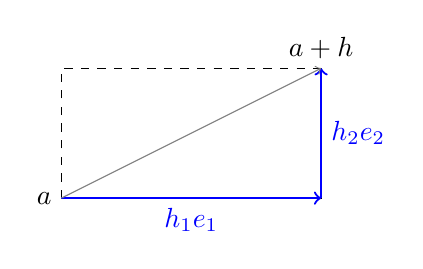
\begin{tikzpicture}[scale=1.1]
\draw[dashed] (0,0) rectangle (3,1.5);
\draw[->,blue,thick] (0,0)--(3,0) node[midway,below] {$h_1e_1$};
\draw[->,blue,thick] (3,0)--(3,1.5) node[midway,right] {$h_2e_2$};
\draw[->,gray] (0,0)--(3,1.5);
\node[left] at (0,0) {$a$}; \node[above] at (3,1.5) {$a+h$};
\end{tikzpicture}
\end{center}
The continuous-partials proof walks from $a$ to $a+h$ one coordinate
at a time. Each segment admits the one-variable mean value theorem.
All intermediate points remain within $\|h\|$ of $a$, so continuity
of the finitely many partials supplies one error bound for all segments.
That common neighborhood is what upgrades coordinate information to a
uniform first-order approximation.
\begin{theorem}[Continuous partial derivatives]
\label{thm:c1-implies-differentiable}
Let $U\subseteq\R^n$ be open.  If all partial derivatives of
\[
f:U\longrightarrow\R^m
\]
exist on a neighborhood of $a$ and are continuous at $a$, then $f$ is
differentiable at $a$ and its derivative is represented in standard
coordinates by $J_f(a)$; explicitly $Df(a)h=J_f(a)h$.
\end{theorem}
\begin{proof}
By \cref{prop:componentwise-differentiability}, it is enough to consider a
real-valued component. Choose $r>0$ so that $B(a,r)$ lies in the neighborhood
where all partial derivatives exist. Telescope the increment from $a$ to
$a+h$ along the coordinate polygonal path. Put
\[
p_0=a,
\qquad
p_j=a+h_1e_1+\cdots+h_je_j
\qquad(1\leq j\leq n).
\]
If $\|h\|_2<r/\sqrt n$, every point $q$ on one of these segments satisfies
\[
\|q-a\|_2\leq |h_1|+\cdots+|h_n|
\leq\sqrt n\,\|h\|_2<r.
\]
Thus the entire coordinate polygonal path lies in $B(a,r)$. If
$h_j=0$, that segment contributes zero; set $a_j=p_{j-1}$ and do not
apply the Mean Value Theorem. For $h_j\ne0$, applying
the one-variable Mean Value Theorem to the function that varies only its
\(j\)th coordinate gives a point
\[
a_j=p_{j-1}+t_jh_je_j
\qquad(0<t_j<1)
\]
such that
\[
f(a+h)-f(a)
=
\sum_{j=1}^{n}
\frac{\partial f}{\partial x_j}(a_j)h_j.
\]
Each \(a_j\) tends to \(a\) with \(h\).  Subtract the same sum with \(a_j\)
replaced by \(a\).  Given \(\eps>0\), continuity of the partial derivatives
makes the absolute value of the difference at most
\[
\eps\sum_{j=1}^{n}\abs{h_j}
\leq
\eps\sqrt n\norm h.
\]
This is the required remainder estimate.  Apply it componentwise.
\end{proof}

\begin{definition}[Class $C^1$]
A differentiable map on an open set is of class
\[
C^1
\]
when its derivative is continuous as a map into the finite-dimensional space
of linear maps.
\end{definition}

Here $Df:U\to\mathcal L(\R^n,\R^m)$ is itself a function, with
linear maps as values. Its continuity at $a$ means
$\|Df(x)-Df(a)\|_{\mathrm{op}}\to0$.
\begin{proposition}[$C^1$ and continuous partials]
A map $f:U\to\R^m$ is $C^1$ if and only if all its first scalar
partial derivatives exist and are continuous on $U$.
\end{proposition}
\begin{proof}
Continuous partials give differentiability by
\cref{thm:c1-implies-differentiable}. Continuity of every matrix entry is
equivalent to operator-norm continuity because matrix space is finite
dimensional. Conversely a continuous derivative has continuous entries
$\partial_j f_i$, by coordinate evaluation.
\end{proof}
\begin{example}[Differentiable need not mean $C^1$]
Reuse $\phi(t)=t^2\sin(1/t)$ for $t\ne0$, $\phi(0)=0$, from Chapter~8,
and put $f(x,y)=\phi(x)$. At zero,
$|f(h)|\leq h_1^2\leq\|h\|^2$, so $Df(0,0)=0$.
Away from $x=0$ the usual rules apply; at every $(0,y)$ the same remainder
bound proves differentiability. But for $x\ne0$,
$\partial_xf=2x\sin(1/x)-\cos(1/x)$, which does not approach zero.
Thus $f$ is differentiable everywhere and is not $C^1$ near the origin.
\end{example}




If a total derivative exists, \cref{prop:derivative-directional} determines
its values on every basis vector. A linear map is determined by those
values, so the partial derivatives supply the \emph{only possible} derivative
$L(h)=J_f(a)h$. Computing this candidate is not a proof of differentiability.
\begin{center}
\fbox{\parbox{.88\linewidth}{\textbf{How to find the total derivative.}
\begin{enumerate}[label=\arabic*.]
\item Compute the partial derivative functions and evaluate them at $a$.
\item Assemble their columns into the candidate matrix $J_f(a)$.
\item Justify differentiability: use nearby partials continuous at $a$
(\cref{thm:c1-implies-differentiable}), the derivative rules and chain
rule, or a direct estimate of the Fr\'echet remainder at an exceptional point.
\item Only then conclude $Df(a)h=J_f(a)h$.
\end{enumerate}}}
\end{center}
For scalar output this reads $Df(a)h=\nabla f(a)\cdot h$.
The gradient is the Euclidean vector representing the derivative covector;
the intrinsic derivative is the linear functional, not that vector.
In the earlier computation of $(xe^y,x^2+y^2)$, the two partial functions
produce the columns and their continuity justifies the derivative.

\begin{example}[Continuous with partials, but not differentiable]
\label{ex:continuous-partials-not-total}
Set $f(0,0)=0$ and $f(x,y)=x^3/(x^2+y^2)$ elsewhere. The bound
\[
|f(x,y)|\leq |x|\leq\sqrt{x^2+y^2}
\]
proves continuity at zero. On the axes $f(t,0)=t$ and $f(0,t)=0$,
so $\partial_xf(0)=1$, $\partial_yf(0)=0$. The only candidate is
$L(h,k)=h$. But $f(t,t)=t/2$ for $t\ne0$, and hence
\[
\frac{|f(t,t)-L(t,t)|}{\|(t,t)\|}=\frac1{2\sqrt2}.
\]
The normalized error does not tend to zero. Without absolute values the
quotient is $-1/(2\sqrt2)$ for $t>0$ and has the opposite sign for
$t<0$; either one-sided approach disproves differentiability.
\end{example}
The earlier example $xy/(x^2+y^2)$ showed that partials alone need not
even imply continuity. This example shows that adding continuity still
does not prove total differentiability. By contrast, nearby partials
continuous at the point do suffice. Partials test coordinate directions;
differentiability requires one linear approximation controlling all
sufficiently small increments at once.

\begin{example}[A direct remainder estimate]
Define $f(0,0)=0$ and, away from the origin,
\[
f(x,y)=\frac{x^2y^2}{x^2+y^2}.
\]
The candidate derivative at the origin is zero.  Since
$4x^2y^2\leq(x^2+y^2)^2$,
\[
\frac{\abs{f(x,y)}}{\norm{(x,y)}}
\leq\frac14\norm{(x,y)}\longrightarrow0.
\]
Hence $f$ is differentiable at the origin by the definition, even without
first proving continuity of its nearby partial derivatives.
\end{example}

The counterexamples form a hierarchy of increasingly demanding tests:
\[
\begin{gathered}
\text{partials}\ <\ \text{all directional derivatives}\\
<\ \text{linear directional data}\ <\ \text{uniform linear approximation}.
\end{gathered}
\]
Here each step means a stronger requirement, not a numerical inequality.
Partials test coordinate lines only. Directional derivatives test each
fixed line, but their values might not depend linearly on direction.
Even linear directional data can fail to control directions that change
with the size of the increment. Differentiability requires one remainder
estimate valid for all sufficiently small increments simultaneously.
\begin{remark}[The same example tests all directions]
For the function in \cref{ex:continuous-partials-not-total} and $v\ne0$,
\[
D_vf(0)=\frac{v_1^3}{v_1^2+v_2^2}.
\]
All directional derivatives exist, but they are not linear in $v$:
the values on $e_1,e_2,e_1+e_2$ are $1,0,1/2$.
They cannot be the values of one linear map $Df(0)$.
\end{remark}







\begin{example}[Even linear directional data can fail]
Let $h(0,0)=0$ and $h(x,y)=x^3y/(x^4+y^2)$ elsewhere.
Since $2|x^2y|\leq x^4+y^2$, $|h(x,y)|\leq|x|/2$, so $h$ is continuous
at zero. For $v=(a,b)$ with $b\ne0$,
\[
\frac{h(ta,tb)}t=\frac{t a^3b}{t^2a^4+b^2}\longrightarrow0;
\]
for $b=0$ it is identically zero. Every directional derivative is therefore
zero; hence $v\mapsto D_vh(0)$ is the zero linear functional. But $h(x,x^2)=x/2$ for $x\ne0$, and
$|h(x,x^2)|/\|(x,x^2)\|\to1/2$. Total differentiability requires
uniform first-order control over all increments, including curved approaches.
\end{example}

In the preceding example $h_t=(t,t^2)$ tends to zero while its direction
changes with $t$. Fixed-line tests do not control this approach.
For a proposed linear map $L$, directional information may give
$[f(a+tv)-f(a)]/t\to Lv$ for each fixed unit $v$, with the allowed size
of $t$ depending on $v$. Differentiability requires a single neighborhood:
\[
\begin{gathered}
\forall\eps>0\ \exists\delta>0\ \forall\|v\|=1\ \forall\,0<|t|<\delta:\\
\left\|\frac{f(a+tv)-f(a)}t-Lv\right\|<\eps.
\end{gathered}
\]
Indeed every nonzero increment has the form $h=tv$ with $v$ unit;
this is exactly the normalized remainder condition.


\Needspace{25\baselineskip}
For a scalar graph $z=f(x,y)$ at $a=(a_1,a_2)$,
Fr\'echet differentiability reads
$f(a+h)=f(a)+Df(a)h+o(\|h\|)$. Its linear map is $Df(a)$;
the affine graph of $h\mapsto f(a)+Df(a)h$ is the tangent plane
\[
z-f(a_1,a_2)=f_x(a_1,a_2)(x-a_1)+f_y(a_1,a_2)(y-a_2).
\]
The derivative is a map, whereas this plane is a set of points in $\R^3$.

\begin{example}[A surface and its affine approximation]
Let $f(x,y)=x^2+xy+2y^2$ and $a=(1,0)$. Then $f(a)=1$ and
$Df(a)(h,k)=2h+k$. The tangent plane is the affine graph
$z=1+2(x-1)+y$. The exact remainder is
\[
f(1+h,k)-1-(2h+k)=h^2+hk+2k^2,
\qquad |h^2+hk+2k^2|\leq\tfrac52(h^2+k^2).
\]
At $(h,k)=(0.01,0.01)$ the linear increment is $0.03$ and the remainder
is $0.0004$, compared with $\|(h,k)\|\approx0.01414$.
Dividing the bound by the increment norm gives a quantity tending to zero.
\begin{center}
\begin{tikzpicture}[x={(2.4cm,-.75cm)},y={(-2cm,-.65cm)},z={(0cm,1.4cm)}]
% A broad oblique view: the two planar directions are visually independent.
\filldraw[fill=orange!25,draw=orange!75!black,thick]
(.5,-.5,-.5)--(1.5,-.5,1.5)--(1.5,.5,2.5)--(.5,.5,.5)--cycle;
\foreach \v in {-.5,-.25,0,.25,.5}{
\draw[blue!65] plot[domain=.5:1.5,samples=24] (\x,\v,{\x*\x+\x*\v+2*\v*\v});}
\foreach \u in {.5,.75,1,1.25,1.5}{
\draw[blue!65] plot[domain=-.5:.5,samples=24] (\u,\x,{\u*\u+\u*\x+2*\x*\x});}
\coordinate (A) at (1,0,1);
\coordinate (P) at (1.45,-.4,1.5);
\coordinate (B) at (1.45,-.4,1.8425);
\fill (A) circle(2pt);
\draw[thin] (A)--++(-1.0cm,.1cm) node[left,fill=white,inner sep=1pt] {contact $(a,f(a))$};
\draw[red!80!black,very thick] (P)--(B);
\fill[red!80!black] (P) circle(1.3pt) (B) circle(1.3pt);
\draw[red!80!black] ($(P)!.5!(B)$)--++(.7cm,0cm)
node[right,fill=white,inner sep=1pt] {remainder};
\draw[dashed,gray] (1.45,-.4,0)--(P);
\draw[->,thick] (1,0,0)--(1.45,-.4,0) node[midway,below] {$h$};
\node[left] at (1,0,0) {$a$};
\draw[orange!70!black] (.6,-.45,-.25)--++(.2cm,-.55cm)
node[below] {affine plane $z=1+2(x-1)+y$};
\draw[blue] (1.5,.5,3.5)--++(.5cm,.25cm) node[right] {$z=f(x,y)$};
% Separate direction key, parallel to the actual projection axes.
\begin{scope}[x={(1cm,0cm)},y={(0cm,1cm)}]
\coordinate (O) at (-1.4,-1.45);
\draw[->] (O)--++(.72,-.225) node[right] {$x$};
\draw[->] (O)--++(-.6,-.195) node[left] {$y$};
\draw[->] (O)--++(0,.75) node[above] {$z$};
\end{scope}
\end{tikzpicture}
\end{center}
The orange plane and blue graph meet at the marked contact point. At a
nearby input $a+h$, the red vertical segment measures their discrepancy,
$h_1^2+h_1h_2+2h_2^2$; scaling $h$ by $t$ scales this error by $t^2$.
The blue mesh therefore bends away from the plane quadratically. $Df(a)$ is the
linear part acting on $(h,k)$; adding $f(a)$ produces the affine graph.
\end{example}

\section{Higher Derivatives and Local Estimates}

The one-variable Mean Value and Taylor theorems describe a function by its
successive local derivatives. In \(\R^n\), restrict the function to a line
segment and apply the Part~I theorem. The resulting coefficients are
evaluations of multilinear derivatives on the segment direction.

\begin{definition}[Convex subset]\label{def:convex-subset}
Extending the Euclidean definition in \cref{def:euclidean-convexity},
a subset $C$ of a real vector space $V$ is \textbf{convex} if
\[
(1-t)x+ty\in C
\]
for every $x,y\in C$ and every $0\leq t\leq1$. The interval property used
in Chapter~8 is exactly the one-dimensional special case.
\end{definition}

\begin{proposition}[Normed-space balls are convex]
\label{prop:normed-balls-convex}
Every open or closed ball in a normed real vector space is convex.
\end{proposition}
\begin{proof}
If $x,y\in\overline B(a,r)$ and $0\leq t\leq1$, then
\[
\begin{aligned}
\|(1-t)x+ty-a\|
&=\|(1-t)(x-a)+t(y-a)\|\\
&\leq(1-t)\|x-a\|+t\|y-a\|\\
&\leq r.
\end{aligned}
\]
Thus $\overline B(a,r)$ is convex. If $x,y\in B(a,r)$, the last bound is
strict because both endpoint distances are strictly less than $r$, proving
the open-ball case.
\end{proof}

\begin{theorem}[Scalar mean-value equality]\label{thm:scalar-multivariable-mvt}
For differentiable $f:U\subseteq\R^n\to\R$ on open $U$ and
$[x,y]\subset U$, there is $t\in(0,1)$ such that
\[
f(y)-f(x)=Df(x+t(y-x))(y-x).
\]
\end{theorem}
\begin{proof}
Apply the ordinary mean value theorem to $g(t)=f(x+t(y-x))$ on $[0,1]$;
the chain rule gives $g'(t)=Df(x+t(y-x))(y-x)$.
\end{proof}
Scalar output admits this exact intermediate-point equality.
For vector-valued functions there need not be a single intermediate point
giving the scalar mean-value equality. For $c(t)=(\cos t,\sin t)$ on
$[0,2\pi]$, the endpoint difference is zero but $c'(t)$ is never zero.
A norm estimate still bounds the change between endpoints.

\begin{theorem}[Mean-value estimate]
\label{thm:multivariable-mvt}
Let $U\subseteq\R^n$ be open, let $f:U\to\R^m$ be differentiable, and suppose
the segment from $x$ to $y$ lies in $U$.  If
\[
\norm{Df((1-t)x+ty)}_{\mathrm{op}}\leq M
\qquad(0\leq t\leq1),
\]
then
\[
\norm{f(y)-f(x)}\leq M\norm{y-x}.
\]
\end{theorem}
\begin{proof}
If $f(y)\ne f(x)$, put
\[
u=\frac{f(y)-f(x)}{\norm{f(y)-f(x)}}
\]
The choice of this unit vector is made so that
\[
u\cdot(f(y)-f(x))
=\frac{\|f(y)-f(x)\|^2}{\|f(y)-f(x)\|}
=\|f(y)-f(x)\|.
\]
Thus one scalar projection captures the full length of the difference.
Keep $u$ fixed while applying the one-variable Mean Value Theorem to
\[
t\longmapsto u\cdot f((1-t)x+ty).
\]
For some $c\in(0,1)$,
\[
\norm{f(y)-f(x)}
=
u\cdot Df((1-c)x+cy)(y-x).
\]
Cauchy--Schwarz and the operator-norm bound prove the assertion.  The zero
case is immediate.
\end{proof}

\begin{corollary}[Local Lipschitz continuity]
If $U$ is convex and $\|Df(x)\|_{\mathrm{op}}\leq M$ on $U$, then
$f$ is $M$-Lipschitz on $U$. Every $C^1$ map is locally Lipschitz.
\end{corollary}
\begin{proof}
Convexity keeps the segment between any $x,y\in U$ in $U$, so
\cref{thm:multivariable-mvt} applies. For a $C^1$ map, continuity of
$Df$ at any $a$ supplies a ball in $U$ where
$\|Df(x)\|_{\mathrm{op}}\leq\|Df(a)\|_{\mathrm{op}}+1$. Apply the first assertion
on that convex ball, using \cref{prop:normed-balls-convex}. A bound outside
the connecting segment would not suffice.
\end{proof}

\begin{proposition}[Differentiating limits of maps]\label{prop:differentiate-map-limits}
Let $f_k:U\subseteq\R^n\to\R^m$ be $C^1$ on open $U$, with
$\overline B(a,r)\subset U$, $r>0$. Let
$A:\overline B(a,r)\to\mathcal L(\R^n,\R^m)$. Suppose $f_k(a)$ converges and
$Df_k\to A$ uniformly in operator norm on this closed ball. Then $f_k$
converges uniformly there to a map $f$, and $Df=A$ on $B(a,r)$.
\end{proposition}
\begin{proof}
Anchor the functions at $a$ and control their increments by the derivatives.
The closed ball is convex by \cref{prop:normed-balls-convex}, so every segment
from $a$ to $x\in\overline B(a,r)$ stays in the ball. The mean-value estimate gives
\[
\|f_k(x)-f_l(x)\|\leq\|f_k(a)-f_l(a)\|
+r\sup_{z\in\overline B(a,r)}\|Df_k(z)-Df_l(z)\|.
\]
Thus the functions are uniformly Cauchy; completeness gives a uniform limit.
The map $A:\overline B(a,r)\to\mathcal L(\R^n,\R^m)$ is continuous by
the uniform-limit theorem, using finite-dimensional coordinates on the target.
Fix $x\in B(a,r)$ and put $\eta=r-\|x-a\|>0$. If $\|h\|<\eta$, then
$\|x+th-a\|<r$ for $0\leq t\leq1$, so the segment stays in the ball. Apply
the mean-value estimate to $z\mapsto f_k(z)-A(x)z$ to obtain
\[
\|f_k(x+h)-f_k(x)-A(x)h\|
\leq\sup_{0\leq t\leq1}\|Df_k(x+th)-A(x)\|\,\|h\|.
\]
Set
\[
e_k=\sup_{z\in\overline B(a,r)}\|Df_k(z)-A(z)\|_{\mathrm{op}}
\longrightarrow0.
\]
The triangle inequality gives the uniform comparison
\[
\sup_{0\leq t\leq1}\|Df_k(x+th)-A(x)\|_{\mathrm{op}}
\leq e_k+\sup_{0\leq t\leq1}\|A(x+th)-A(x)\|_{\mathrm{op}}.
\]
For fixed $h$, letting $k\to\infty$ therefore gives
\[
\|f(x+h)-f(x)-A(x)h\|
\leq\sup_{0\leq t\leq1}\|A(x+th)-A(x)\|_{\mathrm{op}}\,\|h\|.
\]
Now let $h\to0$. Since $\|th\|\leq\|h\|$, continuity of $A$ at $x$
makes the remaining supremum tend to zero. Hence $Df(x)=A(x)$.
\end{proof}
A common derivative bound on a convex neighborhood of a compact set gives
a common Lipschitz bound on that set, hence equicontinuity. With uniform
boundedness, \cref{thm:finite-arzela-ascoli} then gives subsequence compactness.


\Needspace{10\baselineskip}
\begin{definition}[Higher derivatives]\label{def:multivariable-higher-derivatives}
Let $V,W$ be finite-dimensional real normed spaces, $U\subseteq V$ open,
and $f:U\to W$ differentiable. Define inductively
\[
D^0f=f,
\qquad
D^{k+1}f(a)=D(D^kf)(a),
\]
when the right side exists. For $V=\R^n$ and $W=\R^m$, the first two
derivatives initially have the types
\[
Df(a)\in\mathcal L(\R^n,\R^m),\qquad
D(Df)(a)\in\mathcal L\bigl(\R^n,\mathcal L(\R^n,\R^m)\bigr).
\]
The canonical identification sends a linear map $A:V\to\mathcal L(V,W)$
to the bilinear map $(h,k)\mapsto(Ah)(k)$; its inverse sends a bilinear
map $B$ to $h\mapsto B(h,\,\cdot\,)$. Neither construction chooses a basis.
Recall $\mathcal L(V,W)$ from \cref{def:linear-map-space}. Since
$Df:U\to\mathcal L(V,W)$, its derivative satisfies
\[
D(Df)(a):V\to\mathcal L(V,W),\qquad
D^2f(a)[h,k]=(D(Df)(a)h)(k).
\]
This is linear in $h$ because $D(Df)(a)$ is linear, and in $k$ because
each output is itself a linear map. Thus it is bilinear in the sense of
\cref{sec:dual-multilinear}. Inductively, evaluate a linear-map-valued
derivative on its first argument and then on the remaining arguments to
obtain $D^kf(a):V^k\to W$. Its coefficients in bases form a finite array;
continuity and differentiation of that array use the equivalent finite-dimensional norms.  The map is of class $C^k$ when all derivatives through order $k$ exist and are continuous.
\end{definition}

\paragraph{Differentiate the base point, not the increment.}
For fixed $a$, the map $L_a(h)=Df(a)h$ is linear in $h$, and indeed
$DL_a(h)=L_a$. But the second derivative differentiates a different map:
\[
g=Df:U\to\mathcal L(V,W),\qquad x\longmapsto Df(x).
\]
It varies the base point $x$. Its derivative $Dg(a):V\to\mathcal L(V,W)$
measures how the first derivative changes as that point moves. After evaluation,
\[
D^2f(a)[h,k]=(Dg(a)h)(k).
\]
Here $h$ moves the base point and $k$ is the vector on which the changed
first derivative is evaluated. In particular,
\[
Df(a)\in\mathcal L(V,W),\qquad
D^2f(a)\in\mathcal L^2(V;W),
\]
where $\mathcal L^2(V;W)$ denotes the space of bilinear maps $V\times V\to W$.
For scalar-valued $f$, $Df(a)$ is a linear functional on $V$, whereas
$D^2f(a)$ is a bilinear form on $V\times V$. These are different object types.
\begin{example}[A constant derivative and a changing derivative]
If $f(x)=Lx$, then $Df(a)=L$ at every base point. The map $a\mapsto Df(a)$
is constant, so $D^2f(a)=0$, even when $L\ne0$.
For $f(x)=x^2$, $Df(a)h=2ah$ is linear in $h$ at fixed $a$, but
\[
Df(a+k)h-Df(a)h=2kh,\qquad D^2f(a)[k,h]=2kh.
\]
The two independent slots record base-point motion and evaluation.
\end{example}
In general, $D^{k+1}f$ differentiates the function $x\mapsto D^kf(x)$
of the base point. Each differentiation introduces one new independent slot.

For a $k$-linear map $B:V^k\to W$ we use the multilinear operator norm
\[
\|B\|=\sup_{\|v_1\|\leq1,\ldots,\|v_k\|\leq1}\|B(v_1,\ldots,v_k)\|,
\qquad \|B(v_1,\ldots,v_k)\|\leq\|B\|\prod_j\|v_j\|.
\]
Finite-dimensional boundedness follows from the coefficient estimates for
multilinear maps in Chapter~10; the inequality follows by scaling each
nonzero input to a unit vector, with zero inputs handled by multilinearity.

The mixed-increment proof below visualizes the two independent directions.
\begin{center}
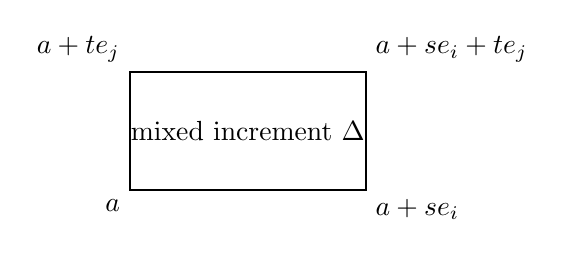
\begin{tikzpicture}
\draw[thick] (0,0) rectangle (3,1.5);
\node[below left] at (0,0) {$a$};
\node[below right] at (3,0) {$a+se_i$};
\node[above left] at (0,1.5) {$a+te_j$};
\node[above right] at (3,1.5) {$a+se_i+te_j$};
\node at (1.5,.75) {mixed increment $\Delta$};
\end{tikzpicture}
\end{center}
\begin{theorem}[Equality of mixed partials]
\label{thm:schwarz}
Let $U\subseteq\R^n$ be open and let $f:U\to\R$ have continuous second
partial derivatives.  Then
\[
\frac{\partial^2f}{\partial x_i\partial x_j}(a)
=
\frac{\partial^2f}{\partial x_j\partial x_i}(a).
\]
\end{theorem}
\begin{proof}
Compute the same rectangular increment in both orders.
For $i=j$ there is nothing to prove. Otherwise choose small positive
$s,t$ so the entire coordinate rectangle is in $U$, and write
\[
\Delta=f(a+se_i+te_j)-f(a+se_i)-f(a+te_j)+f(a).
\]
Apply the mean value theorem to
$u\mapsto f(a+ue_i+te_j)-f(a+ue_i)$ on $[0,s]$. For some
$\xi\in(0,s)$,
\[
\Delta=s\{\partial_i f(a+\xi e_i+te_j)-\partial_i f(a+\xi e_i)\}.
\]
Apply it again, now to $v\mapsto\partial_i f(a+\xi e_i+ve_j)$
on $[0,t]$. For some $\eta\in(0,t)$ this yields
$\Delta/(st)=\partial_j\partial_i f(a+\xi e_i+\eta e_j)$.
Reversing the two initial differences instead gives, for possibly different
$\xi',\eta'$, $\Delta/(st)=\partial_i\partial_j
f(a+\xi'e_i+\eta'e_j)$. Both points tend to $a$ as $s,t\to0^+$.
Continuity of the two mixed partials equates their limits. A single
choice of positive shrinking rectangles suffices to compare their values at $a$.
\end{proof}

\begin{definition}[Hessian and critical points]
Let $f:U\subseteq\R^n\to\R$ be differentiable at $a\in U$, with $U$ open.
If $f$ is of class $C^2$, its \textbf{Hessian} at $a$ is the matrix
\[
h_f(a)=
\left(\frac{\partial^2f}{\partial x_i\partial x_j}(a)\right)_{i,j=1}^n.
\]
Under the standard coordinate identification,
\[
D^2f(a)[h,k]=h^{\mathsf T}h_f(a)k.
\]
By \cref{thm:schwarz}, the Hessian is symmetric.  A point $a\in U$ is a
\textbf{critical point} of a differentiable scalar-valued function when
\[
Df(a)=0,
\]
or equivalently when $\nabla f(a)=0$.
\end{definition}

\begin{proposition}[First-order necessary condition]\label{prop:first-order-extremum}
Let $U\subseteq\R^n$ be open and $f:U\to\R$ differentiable at $a\in U$.
If $a$ is a local maximum or minimum, then $Df(a)=0$.
\end{proposition}
\begin{proof}
Fix $v\in\R^n$. For sufficiently small $t$ of both signs, $a+tv\in U$.
The scalar function $g_v(t)=f(a+tv)$ has a local extremum at the interior
point $0$. The one-variable necessary condition gives
$0=g_v'(0)=Df(a)v$. Since $v$ was arbitrary, $Df(a)=0$.
\end{proof}
Interior matters because both signs of $t$ must be available. Optimization
therefore begins with critical points, but they are only candidates.
The definite second-order tests below are sufficient for classification;
semidefinite cases can be inconclusive.

\paragraph{Compute the Hessian before evaluating its two inputs.}
For scalar $f$, first compute the partial derivative \emph{functions}
$\partial_jf$. Differentiate each of these functions again, freezing all
other coordinates, to obtain $h_f(a)=(\partial_i\partial_jf(a))_{i,j}$.
Continuous second partials justify $C^2$ regularity by applying the
continuous-partials criterion to $f$ and to its derivative's entries.
Once twice differentiability is justified, expanding both inputs in the
standard basis gives
\[
D^2f(a)[h,k]=\sum_{i,j}h_i k_jD^2f(a)[e_i,e_j]
=\sum_{i,j}h_i(\partial_i\partial_j f)(a)k_j=h^{\mathsf T}h_f(a)k.
\]
There are two independently variable input slots. The diagonal value
$h^{\mathsf T}h_f(a)h$ is a quadratic expression obtained by repeating
one input; it is a use of the bilinear map, not its full two-slot formula.

For a $C^2$ map $f=(f_1,\ldots,f_m):U\to\R^m$, compute one scalar
Hessian per output component. Then
\[
D^2f(a)[h,k]=
\begin{pmatrix}h^{\mathsf T}h_{f_1}(a)k\\\vdots\\h^{\mathsf T}h_{f_m}(a)k\end{pmatrix}\in\R^m.
\]
There is no single ordinary Hessian matrix representing all of this
vector-valued bilinear map; there are $m$ two-index coefficient arrays.

\begin{example}[Two directions versus a repeated direction]
For $f(x,y)=x^2+3xy$ and $a=(a_1,a_2)$, the first derivative is the
linear map
\[
Df(a)h=(2a_1+3a_2)h_1+3a_1h_2.
\]
Its coefficient functions are $2x+3y$ and $3x$.
Differentiating again gives the constant Hessian
$h_f=\left(\begin{smallmatrix}2&3\\3&0\end{smallmatrix}\right)$.
The polynomial rules justify smoothness, and the preceding calculation
gives the second derivative at every $a$:
\[
D^2f(a)[h,k]=2h_1k_1+3h_1k_2+3h_2k_1.
\]
This is bilinear and symmetric: interchanging $h,k$ preserves its value.
For $h=(1,0)$ and $k=(0,1)$ it gives $3$, whereas
$D^2f(a)[h,h]=2$. The diagonal specialization is the quadratic expression
$2h_1^2+6h_1h_2$ in one direction; it is not the two-input bilinear map.
\end{example}
\Needspace{13\baselineskip}
\begin{example}[A vector-valued second derivative]
\label{ex:vector-second-differential}
For $f(x,y)=(x^2+3xy,y^2)$, the first derivative sends $h$ to
\[
Df(a)h=((2a_1+3a_2)h_1+3a_1h_2,\,2a_2h_2).
\]
The second derivative is the bilinear map $\R^2\times\R^2\to\R^2$
given by
\[
D^2f(a)[h,k]=(2h_1k_1+3h_1k_2+3h_2k_1,\,2h_2k_2).
\]
Its two components have Hessians
$\left(\begin{smallmatrix}2&3\\3&0\end{smallmatrix}\right)$ and
$\left(\begin{smallmatrix}0&0\\0&2\end{smallmatrix}\right)$.
Repeating the input gives
$D^2f(a)[h,h]=(2h_1^2+6h_1h_2,2h_2^2)$, a vector rather than a scalar.
\end{example}

\paragraph{Second-order objects at a glance.}
For scalar $C^2$ functions, keep the following distinctions:
\begin{itemize}
\item $D^2f(a)$ is a bilinear map; $h_f(a)$ is its matrix in the
standard basis, with entries $\partial_i\partial_j f(a)$.
\item $D^2f(a)[h,k]$ is a scalar obtained by evaluation on two directions.
\item $D^2f(a)[h,h]=h^{\mathsf T}h_f(a)h$ is quadratic as a function of
$h$. For fixed $h$, it is the second derivative at zero of
$t\mapsto f(a+th)$, as the chain rule below verifies.
\end{itemize}
The second directional derivative is therefore an evaluation of the
second differential when $f$ is $C^2$. Existence of separate directional
derivatives alone does not justify a bilinear second differential.

\paragraph{Higher orders: arrays represent multilinear maps.}
The hierarchy of types is
\[
Df(a):\text{ linear},\quad D^2f(a):\text{ bilinear},\quad
D^3f(a):\text{ trilinear},\quad D^kf(a):\text{ $k$-linear}.
\]
For scalar $f\in C^k(U)$, evaluation on basis vectors and repeated
coordinate differentiation give
\[
\begin{split}
D^kf(a)[h^{(1)},\ldots,h^{(k)}]
={}&\sum_{i_1,\ldots,i_k=1}^n
(\partial_{i_1}\cdots\partial_{i_k}f)(a)
\prod_{j=1}^k h^{(j)}_{i_j}.
\end{split}
\]
Indeed the coefficient on $(e_{i_1},\ldots,e_{i_k})$ is the displayed
iterated partial by the recursive definition; multilinearity expands
arbitrary inputs in those basis vectors. The mixed-partial theorem applied
to lower derivatives permits adjacent differentiation orders to be
interchanged. Adjacent swaps generate all permutations, so $D^kf(a)$
is symmetric: for every permutation $\sigma$ of $\{1,\ldots,k\}$,
\[
D^kf(a)[h_{\sigma(1)},\ldots,h_{\sigma(k)}]
=D^kf(a)[h_1,\ldots,h_k].
\]
Apply the formula componentwise for vector-valued outputs. At order two,
equality of mixed partials expresses symmetry of the bilinear map in a
basis. The Hessian represents that map in coordinates; it does not define
the second derivative independently of $D(Df)$.

Order two has two coefficient indices, hence the ordinary Hessian matrix.
Order three has three indices, order four has four, and so on. For
$k\geq3$ there is no preferred ordinary matrix unless indices are grouped
artificially; the symmetric $k$-linear map keeps the input roles visible.
Complete higher-order arrays are rarely computed by hand beyond low
orders. Applications usually need their symmetry, a norm bound, or values
on a repeated direction.
\begin{example}[Three input slots]
For $f(x,y)=x^3+x^2y$, the nonzero third partials are
$f_{xxx}=6$ and $f_{xxy}=f_{xyx}=f_{yxx}=2$. Thus at every $a$,
\[
\begin{split}
D^3f(a)[u,v,w]={}&6u_1v_1w_1\\
&+2(u_1v_1w_2+u_1v_2w_1+u_2v_1w_1).
\end{split}
\]
Each input appears once in every term, and permutation of the three
inputs leaves the value unchanged. On a repeated input the value is
$6h_1^3+6h_1^2h_2$; dividing by $3!$ recovers the cubic polynomial.
\end{example}

\begin{remark}[Symmetric and alternating multilinearity]\label{rem:symmetric-alternating}
Higher derivatives and differential forms share the multilinear language
of Chapter~10, but impose different symmetry. For scalar $C^k$ functions,
$D^kf(a)$ is symmetric and describes higher-order local variation.
Chapter~13's differential $k$-form $\omega_a$ is alternating and describes
oriented $k$-dimensional measurement. Permuting inputs leaves the former
unchanged; exchanging two inputs changes the latter's sign.
For degree at least two an alternating map vanishes on a repeated-input
tuple, whereas $D^kf(a)[h,\ldots,h]$ gives the Taylor term.
\end{remark}

\begin{proposition}[Bilinear differentiation]\label{prop:bilinear-derivative}
Let $V,W,Z$ be finite-dimensional normed spaces and $B:V\times W\to Z$
bilinear with $\|B(u,v)\|\leq C\|u\|\|v\|$. Then
\[
DB(u,v)[p,q]=B(p,v)+B(u,q).
\]
If $f:O\to V$ and $g:O\to W$ are differentiable on an open subset of
a finite-dimensional normed space, then
\[
D\bigl(B(f,g)\bigr)(a)h
=B(Df(a)h,g(a))+B(f(a),Dg(a)h).
\]
\end{proposition}
\begin{proof}
On $V\times W$ use $\|(p,q)\|=\sqrt{\|p\|^2+\|q\|^2}$;
the triangle inequality follows from those in the factors and the Euclidean
triangle inequality in $\R^2$. Expand
\[
B(u+p,v+q)-B(u,v)=B(p,v)+B(u,q)+B(p,q).
\]
The first two terms form a bounded linear map of $(p,q)$, with bound
$(C\|v\|+C\|u\|)\|(p,q)\|$. The remainder satisfies
\[
\|B(p,q)\|\leq C\|p\|\|q\|
\leq\tfrac C2\bigl(\|p\|^2+\|q\|^2\bigr)=o(\|(p,q)\|).
\]
This proves differentiability. The pair map $(f,g)$ has derivative
$h\mapsto(Df(a)h,Dg(a)h)$ by its two remainder estimates. Apply the chain rule.
\end{proof}
In particular evaluation $E:\mathcal L(W,Z)\times W\to Z$, $E(A,w)=Aw$,
is bounded bilinear since $\|Aw\|\leq\|A\|_{\mathrm{op}}\|w\|$.

\begin{proposition}[Second-order chain rule]\label{prop:second-chain-rule}
Let $V,W,Z$ be finite-dimensional real normed spaces.
For $C^2$ maps $f:U\subseteq V\to W$ and $g:U_1\subseteq W\to Z$,
where $U,U_1$ are open and $f(U)\subseteq U_1$, we have for $h,k\in V$
\[
\begin{split}
D^2(g\circ f)(a)[h,k]={}&D^2g(f(a))[Df(a)h,Df(a)k]\\
&+Dg(f(a))\bigl[D^2f(a)[h,k]\bigr].
\end{split}
\]
\end{proposition}
\begin{proof}
For fixed $k\in V$, differentiate
$D(g\circ f)(x)k=Dg(f(x))(Df(x)k)$ in direction $h\in V$.
Apply \cref{prop:bilinear-derivative} to the bounded evaluation map
$E(A,w)=Aw$. Its rule differentiates each factor once. The first derivative of the first factor is
$D^2g(f(a))[Df(a)h,\,\cdot\,]$; that of the second is
$D^2f(a)[h,k]$. Their two contributions are exactly the formula.
\end{proof}
Here $Df(a):V\to W$ sends both directions to $W$;
$D^2g(f(a)):W\times W\to Z$ is evaluated on those two images.
The other term first uses $D^2f(a):V\times V\to W$, then
$Dg(f(a)):W\to Z$. Both outputs belong to $Z$. For scalar one-variable
maps and $h=k=1$, this is $(g\circ f)''=g''(f)(f')^2+g'(f)f''$.

Unlike the first-order rule, the second-order rule has two contributions.
The first comes from curvature of the outer map $g$, tested on the two
directions transported by $Df(a)$. The second comes from nonlinear
variation of $f$, carried to the target by $Dg(f(a))$. If $f$ is affine,
the second term vanishes; if $g$ is affine, the first vanishes.
At higher orders, differentiating a term either adds an input to an outer
derivative or differentiates one of its inner factors. The resulting sums
are organized by partitions of the input directions into groups: each
group enters one derivative of $f$, and their outputs enter a derivative
of $g$. We will not need the general combinatorial formula.

\begin{corollary}[Second derivative along a curved path]\label{cor:curved-second-derivative}
If $f:U\subseteq\R^n\to\R$ and $\gamma:I\to U$ are $C^2$, then
\[
(f\circ\gamma)''(t)
=D^2f(\gamma(t))[\gamma'(t),\gamma'(t)]
 +Df(\gamma(t))\gamma''(t).
\]
\end{corollary}
\begin{proof}
Apply \cref{prop:second-chain-rule} to $f\circ\gamma$ and evaluate on
$1,1\in\R$.
\end{proof}
The first term measures second-order variation of $f$ along current velocity;
the second pairs its first derivative with the path's acceleration.
A line $\gamma(t)=a+tv$ has $\gamma''=0$, explaining the simpler identity
$g''(t)=D^2f(a+tv)[v,v]$ for $g(t)=f(a+tv)$.
For $f(x,y)=x^2+y^2$ and $\gamma(t)=(\cos t,\sin t)$,
\[
D^2f(\gamma)[\gamma',\gamma']=2,\qquad
Df(\gamma)\gamma''=2\gamma\cdot(-\gamma)=-2.
\]
Their sum is zero, as it must be since $f\circ\gamma=1$. A curved path
generally contributes more than the Hessian term alone.

The \emph{Taylor polynomial in the increment} $h$ is
\[
T_kf(a;h)=\sum_{j=0}^k\frac1{j!}D^jf(a)[h,\ldots,h],
\]
where the $j=0$ term means $f(a)$. Each $D^jf(a)$ is a symmetric
$j$-linear map; evaluating on $j$ copies of $h$ gives a homogeneous
polynomial of degree $j$ (scaling $h$ by $t$ scales the term by $t^j$).
For scalar output, its first two coordinate terms are
\[
Df(a)h=\sum_i f_{x_i}(a)h_i,\qquad
D^2f(a)[h,h]=h^{\mathsf T}h_f(a)h=\sum_{i,j}f_{x_ix_j}(a)h_ih_j.
\]
Thus in two variables the intrinsic formula reads
\[
\begin{split}
f(a+h)={}&f(a)+f_x(a)h_1+f_y(a)h_2\\
&+\tfrac12\bigl(f_{xx}(a)h_1^2+2f_{xy}(a)h_1h_2+f_{yy}(a)h_2^2\bigr)
+\text{remainder}.
\end{split}
\]
For a fixed direction $v$ and $g(t)=f(a+tv)$, the chain rule repeated
$j$ times gives
\[
g^{(j)}(t)=D^jf(a+tv)[v,\ldots,v],\qquad
g^{(j)}(0)=D^jf(a)[v,\ldots,v].
\]
Only $t$ varies; the direction remains fixed. Each differentiation inserts
one more copy of $v$, since the line has constant velocity and no higher
derivatives. This generalizes the one-variable formula in
the subsection ``\nameref{sec:ordinary-higher-derivatives}.'' The following theorem explains
the remainder by taking $v=h$ and applying one-variable Taylor to $g$.


\Needspace{10\baselineskip}
\begin{theorem}[Taylor's theorem along a segment]
\label{thm:multivariable-taylor}
Let $k\geq0$ be an integer. Let $U\subseteq\R^n$ be open, let $f:U\to\R^m$ be of class $C^{k+1}$, and suppose the segment from $a$ to $a+h$ is in $U$.  If $m=1$, there is
\[
\theta\in(0,1)
\]
such that
\[
f(a+h)
=
\sum_{j=0}^{k}\frac1{j!}D^jf(a)[h,\ldots,h]
+
\frac1{(k+1)!}D^{k+1}f(a+\theta h)[h,\ldots,h].
\]
For vector-valued $f$, this formula holds componentwise, possibly with a
different value of $\theta$ for each component.
\end{theorem}
\begin{proof}
For a scalar component define
\[
g(t)=f(a+th).
\]
Keep $h$ fixed. Always $g'(t)=Df(a+th)h$. If $k\geq1$, the
hypothesis also supplies the second derivative
\[
g''(t)=D^2f(a+th)[h,h].
\]
For $k=0$ only $g'$ is needed.
Each differentiation inserts the same segment direction once more.
Repeated application of the chain rule gives
\[
g^{(j)}(t)=D^jf(a+th)[h,\ldots,h].
\]
Apply the one-variable Taylor theorem \cref{thm:taylor} to $g$ at zero and
evaluate at one.  Do this for each component.
\end{proof}

\begin{corollary}[Taylor error bound and general Peano form]\label{cor:general-peano}
If $f$ is $C^{k+1}$ on a neighborhood of a segment and $\|D^{k+1}f\|\leq M$ there,
then, in Euclidean target norm,
\[
\|f(a+h)-T_kf(a;h)\|\leq\frac{M}{(k+1)!}\|h\|^{k+1}.
\]
If $f$ is only $C^k$ near $a$, $k\geq1$, then
$f(a+h)=T_kf(a;h)+o(\|h\|^k)$.
\end{corollary}
\begin{proof}
For a nonzero remainder vector $R$, fix $u=R/\|R\|$ and apply the
scalar segment theorem to $u\cdot f$. Its remainder is $u\cdot R=\|R\|$,
and $|u\cdot D^{k+1}f[h,\ldots,h]|\leq M\|h\|^{k+1}$.
The zero case is immediate; no common intermediate point for all
components is asserted.
For the Peano assertion follow the proof of \cref{cor:ordinary-peano}:
apply the same projection argument to
$R=f(a+h)-T_kf(a;h)$, using the segment theorem of order $k-1$.
After subtracting the degree-$k$ term, it bounds $\|R\|$ by
\[
\frac{\|h\|^k}{k!}\sup_{0\leq t\leq1}
\|D^kf(a+th)-D^kf(a)\|.
\]
Continuity at $a$ makes the supremum tend to zero.
\end{proof}
The $C^{k+1}$ hypothesis gives a scalar Lagrange remainder along the
segment and a vector norm estimate. The weaker $C^k$ hypothesis suffices
for the Peano error.


\Needspace{8\baselineskip}
\begin{corollary}[Second-order Taylor--Peano formula]
\label{cor:second-peano}
For $f:U\to\R^m$ of class $C^2$ near $a$,
\[
f(a+h)=f(a)+Df(a)h+\tfrac12D^2f(a)[h,h]+o(\|h\|^2).
\]
\end{corollary}
\begin{proof}
Apply the $C^k$ Peano part of \cref{cor:general-peano} with $k=2$. No third derivative is required.
\end{proof}
\begin{example}[Computing a quadratic Taylor polynomial]
For $f(x,y)=e^x\cos y$, first compute the gradient and Hessian:
\[
\nabla f=(e^x\cos y,-e^x\sin y),\qquad
h_f=\begin{pmatrix}e^x\cos y&-e^x\sin y\\-e^x\sin y&-e^x\cos y\end{pmatrix}.
\]
At $a=(0,0)$ these are $(1,0)$ and $\operatorname{diag}(1,-1)$.
For $h=(u,v)$, the coordinate quadratic expression is
$h^{\mathsf T}h_f(0)h=u^2-v^2$. Hence
\[
T_2f(0;h)=1+u+\tfrac12(u^2-v^2),\qquad
e^u\cos v=T_2f(0;h)+O(\|h\|^3).
\]
Indeed the third derivative is continuous and therefore bounded by some
$M$ on a fixed compact ball around zero; the error is at most
$M\|h\|^3/6$ there. With only $C^2$ information the justified conclusion
would instead be $o(\|h\|^2)$. The bilinear Hessian has two input slots;
the polynomial repeats the increment in both.
\end{example}

\paragraph{Coordinate expansion of the Taylor polynomial.}
The polynomial is defined by evaluating multilinear derivatives on the
increment. Multi-indices abbreviate its coordinate expansion.
A multi-index is a tuple $\alpha=(\alpha_1,\ldots,\alpha_n)$
of nonnegative integers, with
\[
|\alpha|=\sum_i\alpha_i,\qquad \alpha!=\prod_i\alpha_i!,\qquad
h^\alpha=\prod_i h_i^{\alpha_i},\qquad
\partial^\alpha=\partial_1^{\alpha_1}\cdots\partial_n^{\alpha_n}.
\]
Expanding $D^jf(a)[h,\ldots,h]$ by multilinearity gives one term for
each ordered choice of $j$ coordinate indices. If index $i$ occurs
$\alpha_i$ times, the same monomial $h^\alpha$ occurs $j!/\alpha!$
times. Symmetry makes their derivative coefficients equal. Consequently
\[
\frac1{j!}D^jf(a)[h,\ldots,h]
=\sum_{|\alpha|=j}\frac{\partial^\alpha f(a)}{\alpha!}h^\alpha.
\]
This is a finite identity for $C^j$ maps, componentwise for vector output;
it does not require analyticity. The Taylor polynomial specifies the
coefficients, the Peano remainder asserts local approximation as $h\to0$,
and the quantitative bound above uses one more bounded derivative.

\subsubsection*{Smoothness and real analyticity}
The distinction in \cref{def:ordinary-analytic,thm:smooth-cutoff} remains
essential in several variables. Here $C^\infty$ means $C^k$ for every
finite $k$, not equality to an infinite Taylor expansion.
\begin{definition}[Real-analytic map]
A scalar function on an open subset of $\R^n$ is real analytic at $a$
if on a neighborhood of $a$ it is represented by a convergent power
series in the coordinates of $h=x-a$. It is real analytic on its domain
if this holds at every point. Vector-valued maps are real analytic when
each scalar component is.
\end{definition}
Here convergent power series means absolute convergence on a sufficiently
small coordinate box. Termwise differentiation is valid on smaller boxes:
choose $0<r<R$ with the closed box of radius $R$ inside it. For a fixed
multi-index $\beta$ of order $q=|\beta|$ and $\alpha\geq\beta$
coordinatewise, put $m=|\alpha|$. Then
\[
\begin{aligned}
\sup_{\|h\|_\infty\leq r}|\partial^\beta(c_\alpha h^\alpha)|
&\leq |c_\alpha|m^q r^{m-q}\\
&=r^{-q}m^q(r/R)^m|c_\alpha|R^m
\leq C_{\beta,r,R}|c_\alpha|R^{|\alpha|},
\end{aligned}
\]
where $C_{\beta,r,R}=r^{-q}\sup_{m\geq0}m^q(r/R)^m<\infty$.
For $q=0$ take $m^0=1$; if $\alpha\not\geq\beta$, the derivative is
zero. The supremum is finite because geometric decay dominates fixed
polynomial growth. Absolute convergence gives
$\sum_\alpha|c_\alpha|R^{|\alpha|}<\infty$, so the M-test proves uniform
convergence of each derivative series on the smaller box. Apply the
differentiating-limits theorem successively in each coordinate. As in
Chapter~8, this proves smoothness and the forced coefficients
$\partial^\alpha f(a)/\alpha!$.
Thus, for sufficiently small $h$,
\[
f(a+h)=\sum_\alpha\frac{\partial^\alpha f(a)}{\alpha!}h^\alpha
=\sum_{j=0}^\infty\frac1{j!}D^jf(a)[h,\ldots,h].
\]
Group terms by $|\alpha|=j$ and use the finite coordinate identity above.
Absolute convergence justifies this grouping of the infinite series.

Analytic implies $C^\infty$, which implies $C^k$ for each finite $k$.
The reverse implications fail, as the one-variable examples composed
with a coordinate projection show. For each \emph{fixed} $k$,
\cref{cor:general-peano} gives $T_kf(a;h)+o(\|h\|^k)$ as $h\to0$.
It supplies no estimate allowing $k\to\infty$ with $h$ fixed.
\begin{example}[A smooth map not recovered by its Taylor series]
Let $f(x_1,\ldots,x_n)=\theta(x_1)$ with $\theta$ from
\cref{thm:smooth-cutoff}. The chain rule with coordinate projection
makes $f$ smooth. A derivative involving another coordinate is zero;
the derivatives using only $x_1$ are derivatives of $\theta$.
Hence $f(0)=0$ and $D^kf(0)=0$ for every $k\geq1$. Its Taylor series
at zero is the zero series, although $f(x)>0$ whenever $x_1>0$.
All derivatives at a point therefore need not determine a smooth map nearby.
\end{example}
The inverse and implicit function arguments below preserve $C^r$
regularity, including $r=\infty$. They do not establish analyticity:
existence of derivatives of every order is not a proof that a Taylor
series converges to the inverse or implicit function.

\paragraph{Higher derivatives of local inverses and implicit graphs.}
The inverse theorem below first constructs a $C^1$ inverse and then gains
derivatives from its first-derivative formula. Writing $g=f^{-1}$, the
identity $g\circ f=\operatorname{id}$ gives
\[
Dg(f(x))=[Df(x)]^{-1},\qquad
Dg=\operatorname{Inv}\circ Df\circ g,
\]
where $\operatorname{Inv}(A)=A^{-1}$ on $GL(\R^n)$. Smoothness of
operator inversion, proved below, makes the available regularity visible:
\[
f\in C^k\ \Longrightarrow\ Df\in C^{k-1}
\ \Longrightarrow\ (x\mapsto[Df(x)]^{-1})\in C^{k-1}.
\]
Composition with $g$ must be justified inductively. Once $g\in C^j$
for $j<k$, the formula for $Dg$ gives $Dg\in C^j$ and hence
$g\in C^{j+1}$. Repeating this reaches $Dg\in C^{k-1}$ and $g\in C^k$.
Here $[Df(x)]^{-1}$ means inversion of a linear map, not differentiation
of an inverse function. The implicit graph is constructed from the local
inverse of $h(x,y)=(x,f(x,y))$ by restricting to $(x,0)$ and projecting
onto the remaining coordinates. These operations preserve $C^k$
regularity, so no separate higher-order existence argument is needed.

\Needspace{13\baselineskip}
\subsubsection*{Using the quadratic term at an extremum}
\begin{corollary}[Second-order test]
\label{cor:second-order-test}
Let $f:U\to\R$ be of class $C^2$ and satisfy
\[
Df(a)=0.
\]
If
\[
D^2f(a)[h,h]>0
\qquad(h\ne0),
\]
then $a$ is a strict local minimum.  If the displayed inequality is reversed,
then $a$ is a strict local maximum.
\end{corollary}
\begin{proof}
On the Euclidean unit sphere, the continuous quadratic form has a positive
minimum: compactness follows from \cref{thm:heine-borel-rn}, and
attainment from \cref{thm:compact-extreme-value}.  Hence
\[
D^2f(a)[h,h]\geq c\norm h^2
\]
for some $c>0$.  The sphere minimum is attained at a nonzero vector, so it is strictly
positive; pointwise positivity alone would not yield this uniform constant
without compactness. By \cref{cor:second-peano}, choose $\|h\|$ small
enough that the absolute remainder is at most $c\|h\|^2/4$. Then
$f(a+h)-f(a)\geq(c/2-c/4)\|h\|^2>0$ for $h\ne0$.  Apply this to $-f$ for the
maximum assertion.
\end{proof}





\begin{remark}[Saddles and inconclusive Hessians]
At a critical point, an indefinite Hessian gives directions $u,v$ with
$D^2f(a)[u,u]>0>D^2f(a)[v,v]$. Taylor expansion along $tu$ and $tv$
then gives values above and below $f(a)$ arbitrarily nearby: a saddle.
For example $x^2-y^2$ has this behavior at zero. A semidefinite Hessian
is generally inconclusive: both $x^4+y^4$ and $x^4-y^4$ have zero Hessian
at zero, but the first has a strict minimum and the second a saddle.
\end{remark}


\begin{example}[Level ellipses and the gradient]
For $f(x,y)=x^2+2y^2$, take $a=(1,1)$ on the level $f=3$.
Then $\nabla f(a)=(2,4)$, and for unit directions
\[
D_{(1,0)}f(a)=2,\qquad
D_{(2,-1)/\sqrt5}f(a)=0,\qquad
D_{(1,2)/\sqrt5}f(a)=2\sqrt5.
\]
The middle direction is tangent to the ellipse; the last is the gradient
direction, which maximizes first-order increase by Cauchy--Schwarz.
\begin{center}
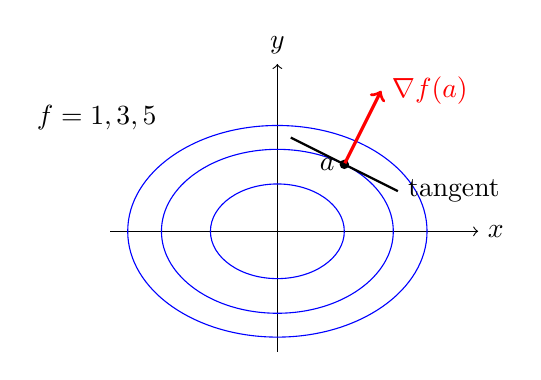
\begin{tikzpicture}[scale=.85]
\draw[->] (-2.5,0)--(3,0) node[right] {$x$};
\draw[->] (0,-1.8)--(0,2.5) node[above] {$y$};
\foreach \r in {1,1.732,2.236}{\draw[blue] (0,0) ellipse[x radius=\r,y radius={\r/sqrt(2)}];}
\fill (1,1) circle(2pt) node[left] {$a$};
\draw[->,red,very thick] (1,1)--(1.55,2.1) node[right] {$\nabla f(a)$};
\draw[thick] (.2,1.4)--(1.8,.6) node[right] {tangent};
\node at (-2.7,1.7) {$f=1,3,5$};
\end{tikzpicture}
\end{center}
More generally, for $a,b>0$ the ellipse $x^2/a^2+y^2/b^2=1$ has
normal $(2x/a^2,2y/b^2)$ at $(x,y)$. At $(x_0,y_0)$ its tangent line is
$x_0x/a^2+y_0y/b^2=1$. The hyperbola $x^2/a^2-y^2/b^2=1$ similarly
has nonzero normal $(2x/a^2,-2y/b^2)$ everywhere, although it has two
components, distinguished by $x>0$ and $x<0$.
\end{example}

\subsection{Convexity and global minima}
The line-segment method also generalizes Chapter~8's convexity theory.
For an open convex $U\subseteq\R^n$, a function $f:U\to\R$ is convex if
\[
f((1-t)x+ty)\leq(1-t)f(x)+tf(y)\qquad(x,y\in U,\ 0\leq t\leq1).
\]
It is strictly convex if the inequality is strict for $x\ne y$ and
$0<t<1$. The tangent affine function will now replace the tangent line.
\begin{proposition}[Criteria for convexity]\label{prop:multivariable-convexity}
For differentiable $f$, convexity is equivalent to
\[
f(y)\geq f(x)+Df(x)(y-x)\qquad(x,y\in U).
\]
For $C^2$ functions it is equivalent to
$D^2f(x)[h,h]\geq0$ for all $x\in U$, $h\in\R^n$;
in coordinates, the Hessian is positive semidefinite everywhere.
\end{proposition}
\begin{proof}
Restrict to $g(t)=f(x+t(y-x))$. Convexity gives
$(g(t)-g(0))/t\leq g(1)-g(0)$ for $0<t<1$; let $t\downarrow0$
to obtain the supporting inequality. Conversely put $z=(1-t)x+ty$,
apply that inequality based at $z$ to $x$ and $y$, and multiply by
$1-t$ and $t$. The derivative terms sum to
$Df(z)((1-t)x+ty-z)=0$, proving convexity.
For $C^2$ functions the restriction has
$g''(t)=D^2f(x+t(y-x))[y-x,y-x]$; the one-variable second-derivative
criterion proves sufficiency. Necessity follows by restricting a convex
$f$ to a small line interval $x+th$ within the open domain and testing at zero.
\end{proof}
If $Df(a)=0$, the supporting inequality gives $f(y)\geq f(a)$ everywhere:
$a$ is a global minimum. For strictly convex $f$ there cannot be two
minimizers, since their midpoint would have a smaller value.
For example $f(x,y)=(x-1)^2+2(y+1)^2$ has Hessian
$\operatorname{diag}(2,4)$ everywhere and its unique critical point
$(1,-1)$ is its unique global minimum. A positive definite Hessian at
one \emph{critical} point gives the earlier local minimum test; a positive
semidefinite Hessian everywhere on a convex domain gives global convexity.


\section{The Contraction Principle}

To solve an inverse or implicit equation, we will rearrange it as
$x=T(x)$ and look for a fixed point. Repeatedly applying $T$ should
improve an approximate solution. A contraction gives existence, uniqueness,
and convergence of these iterates together; completeness keeps their limit
inside the space. This is the tool behind the next section's local
inverse and implicit function theorems.


\begin{definition}[Contraction]
A map
\[
T:X\longrightarrow X
\]
on a metric space is a \textbf{contraction} if
\[
d(Tx,Ty)\leq qd(x,y)
\]
for all $x,y\in X$ and some
\[
0\leq q<1.
\]
\end{definition}

\Needspace{12\baselineskip}
\begin{theorem}[Contraction mapping theorem]
\label{thm:contraction}
A contraction of a nonempty complete metric space has a unique fixed point.  For every
$x_0$, the sequence
\[
x_{n+1}=T(x_n)
\]
converges to it.
\end{theorem}
\begin{proof}
The contraction inequality gives
\[
d(x_{n+1},x_n)\leq q^nd(x_1,x_0).
\]
Thus, for $m>n$,
\[
d(x_m,x_n)\leq\sum_{j=n}^{m-1}d(x_{j+1},x_j)
\leq d(x_1,x_0)\sum_{j=n}^{m-1}q^j
\leq\frac{q^n}{1-q}d(x_1,x_0).
\]
The last bound is independent of $m>n$, proving the Cauchy property. Completeness gives a limit $x$.  Continuity of $T$ implies
\[
T(x)=T(\lim_n x_n)=\lim_n T(x_n)=\lim_n x_{n+1}=x.
\]
If $x,y$ are fixed, then
\[
d(x,y)\leq qd(x,y),
\]
so $x=y$.
\end{proof}

\begin{corollary}[Contractions on a Euclidean open ball]
\label{cor:open-ball-contraction}
Let $r>0$, and suppose
\[
T:B_2(0,r)\longrightarrow\R^n
\]
is Lipschitz with constant $0\leq q<1$ and
\[
\norm{T(0)}<(1-q)r.
\]
Then $T$ maps $B_2(0,r)$ into itself, has a unique fixed point $p$ there,
and
\[
\norm p\leq\frac{\norm{T(0)}}{1-q}<r.
\]
For every $x_0\in B_2(0,r)$, the iteration $x_{j+1}=T(x_j)$ converges to
$p$.
\end{corollary}
\begin{proof}
Put $c=\norm{T(0)}/(1-q)<r$. If $\norm x<r$, then
\[
\norm{T(x)}\leq\norm{T(x)-T(0)}+\norm{T(0)}
\leq q\norm x+(1-q)c<r,
\]
so $T$ is a self-map of the open ball. That ball need not be complete, so
we do not apply the contraction theorem to it. Choose $s$ with
$c<s<r$. For $\norm x\leq s$,
\[
\norm{T(x)}\leq qs+(1-q)c<s.
\]
Thus the closed ball $\overline B_2(0,s)$ is invariant and is complete by
\cref{cor:closed-ball-complete}, so
\cref{thm:contraction} gives a fixed point $p$ in it. Any fixed point in
the open ball is unique by the contraction inequality, and
\[
(1-q)\norm p\leq\norm{T(0)}
\]
gives the asserted bound. Given an arbitrary $x_0$ in the open ball,
choose instead $s$ with $\max\{c,\norm{x_0}\}<s<r$. The same invariant
closed-ball argument then proves convergence of its iterates to $p$.
\end{proof}

The strict inequality is sharp. On $(-1,1)$, the map
$T(x)=(x+1)/2$ has $q=1/2$ and
$|T(0)|=(1-q)r=1/2$, but its only fixed point is the boundary point $1$.

\begin{example}[Solving $x=\cos x$ by iteration]
On $X=[1/2,1]$ with the usual metric, $T(x)=\cos x$ maps $X$ into itself.
Indeed, the elementary-function theory gives
$1/2<\cos1\leq\cos x<1$ there.  The Mean Value Theorem and
$\abs{\sin x}\leq\sin1<1$ give
\[
\abs{T(x)-T(y)}\leq(\sin1)\abs{x-y}.
\]
The closed interval is complete, so the contraction theorem gives a unique
solution in $X$, and the numerical iteration
$x_{n+1}=\cos x_n$ converges to it from every starting point in $X$.
Completeness is used precisely when the Cauchy iterates are asserted to have
a limit. Similar successive approximations will give existence results for
differential equations, integral equations, and problems in functional
analysis.
\end{example}

\paragraph{What each contraction hypothesis contributes.}
The self-map hypothesis keeps every iterate in the space. The factor
$q<1$ makes successive steps shrink geometrically. Completeness places
the Cauchy limit in that same space. For $T(x)=x/2$ on $(0,1)$,
the first two properties hold but the fixed point $0$ is missing, so
completeness cannot be omitted. On $\R$, $T(x)=x+1$ shows why a
Lipschitz factor $1$ is insufficient even in a complete space.

The geometric tail gives usable stopping bounds. For $x_n=T^nx_0$
and the fixed point $p$,
\[
d(x_n,p)\leq\frac{q^n}{1-q}d(x_1,x_0),\qquad
d(x_n,p)\leq\frac{q}{1-q}d(x_n,x_{n-1})\quad(n\geq1).
\]
Indeed every future step is bounded by a successive power of $q$ times
the first remaining step; sum that geometric series and let the far
endpoint tend to $p$. The second bound uses the observed last step,
so it can certify the accuracy during an iteration.
\begin{proposition}[Perturbation of an invertible map]
\label{prop:perturbation}
Let $A,B\in\mathcal L(\R^n)$ and let $A$ be invertible. If
\[
\norm{I-A^{-1}B}_{\mathrm{op}}<1,
\]
then $B$ is invertible.
\end{proposition}
\begin{proof}
Set $T=I-A^{-1}B$. By \cref{prop:neumann-series}, $I-T$ has
inverse $S=\sum_{k=0}^\infty T^k$. Since $B=A(I-T)$, its inverse is
$SA^{-1}$, in that order.
\end{proof}



\section{Inverse and Implicit Functions}

There are two related questions. An inverse problem solves $y=f(x)$ for
$x$ as a function of $y$. An implicit problem solves $f(x,y)=0$ for
one block of variables, say $y$, in terms of the other block $x$.
In each case we first ask whether the linear approximation can solve
for the desired unknowns.


For an invertible operator $T\in\mathcal L(\R^n)$, invertibility is equivalent
to $\det T\ne0$.  In one variable, the corresponding hypothesis
\(f'(a)\ne0\) says that the linear approximation \(h\mapsto f'(a)h\) can
be inverted.  For a map
\[
\R^n\longrightarrow\R^n,
\]
the exact replacement is that \(Df(a)\) is an invertible linear map.  Since
\[
f(a+h)=f(a)+Df(a)h+o(\norm h),
\]
the natural question is whether an invertible best linear approximation
forces $f$ itself to be invertible nearby.  The inverse function theorem
answers yes, locally: close to $a$, the map neither folds space nor collapses
a direction, and nearby points can be recovered uniquely from their images.

Regard $\mathcal L(\R^n)$ as a finite-dimensional normed vector space with
the operator norm. Any equivalent norm gives the same topology and the same
finite-dimensional $C^k$ notion; the operator norm is natural here because
it controls composition and perturbations. Write
\[
\operatorname{GL}(\R^n)
=\{A\in\mathcal L(\R^n):A\text{ is invertible}\}.
\]
Thus $\operatorname{GL}(\R^n)\subseteq\mathcal L(\R^n)$; after a basis is
chosen these operators are represented by the usual invertible matrices.

\begin{lemma}[Smooth inversion of operators]\label{lem:smooth-matrix-inversion}
The set $\operatorname{GL}(\R^n)$ is open in $\mathcal L(\R^n)$, and
\[
\operatorname{Inv}:\operatorname{GL}(\R^n)\longrightarrow
\mathcal L(\R^n),\qquad \operatorname{Inv}(A)=A^{-1},
\]
is smooth. Its derivative is the linear map
\[
D\operatorname{Inv}(A):\mathcal L(\R^n)\longrightarrow
\mathcal L(\R^n),\qquad
D\operatorname{Inv}(A)[h]=-A^{-1}HA^{-1}.
\]
\end{lemma}
\begin{proof}
Fix $A\in\operatorname{GL}(\R^n)$. The estimate
\[
\|A^{-1}(B-A)\|_{\mathrm{op}}
\leq\|A^{-1}\|_{\mathrm{op}}\|B-A\|_{\mathrm{op}}
\]
shows that
\[
\|B-A\|_{\mathrm{op}}<\frac{1}{2\|A^{-1}\|_{\mathrm{op}}}
\quad\Longrightarrow\quad
\|A^{-1}(B-A)\|_{\mathrm{op}}<\frac12<1.
\]
The perturbation result \cref{prop:perturbation} then makes $B$ invertible,
so $\operatorname{GL}(\R^n)$ is open.

We first establish continuity and the local bound used in the derivative
estimate. If
$\norm{A^{-1}(B-A)}_{\mathrm{op}}<1/2$, the geometric series gives
\[
\norm{B^{-1}}_{\mathrm{op}}\leq2\norm{A^{-1}}_{\mathrm{op}}.
\]
The exact resolvent identity
\[
B^{-1}-A^{-1}=B^{-1}(A-B)A^{-1}
\]
then proves $B^{-1}\to A^{-1}$ when $B\to A$.

For $\|h\|_{\mathrm{op}}<1/(2\|A^{-1}\|_{\mathrm{op}})$, the preceding
argument makes $A+h$ invertible. Rearranging
$(A+h)^{-1}(A+h)=I$ first gives
\[
(A+h)^{-1}-A^{-1}=-(A+h)^{-1}HA^{-1}.
\]
Combining the same identity in the opposite order gives the exact remainder
identity
\[
(A+h)^{-1}-A^{-1}+A^{-1}HA^{-1}
=A^{-1}HA^{-1}h(A+h)^{-1}.
\]
The local bound for $(A+h)^{-1}$ makes the right side
$O(\norm h_{\mathrm{op}}^2)$. This proves the displayed derivative formula.
Operator composition
$(R,S)\mapsto RS$ is bilinear, hence smooth, so
\[
(A,h)\longmapsto-\operatorname{Inv}(A)h\operatorname{Inv}(A)
\]
is as differentiable in $A$ as $\operatorname{Inv}$ itself. Starting from
$C^1$ and applying this observation inductively proves $C^j$ regularity for
every finite $j$, and therefore smoothness.
\end{proof}

\begin{definition}[Diffeomorphisms]
\label{def:diffeomorphism}
Let $U\subseteq\R^n$ and $V\subseteq\R^m$ be open. A bijection
$f:U\to V$ is a \textbf{$C^k$ diffeomorphism} if both $f$ and $f^{-1}$
are of class $C^k$. When $k=\infty$, it is a \textbf{smooth
diffeomorphism}. A map is a \textbf{local $C^k$ diffeomorphism at $a$}
if its restriction to some open neighborhood of $a$ is a $C^k$
diffeomorphism onto an open set.
\end{definition}

The correction map $T_y(x)=x-Df(a)^{-1}(f(x)-y)$ comes from solving
the affine model. If $f(x)=f(a)+B(x-a)$ with $B$ invertible, then
\[
T_y(x)=a+B^{-1}(y-f(a)),
\]
independent of $x$ and exactly the solution of $f(x)=y$. For a nonlinear
map, source and target translations move $a$ and $f(a)$ to zero, while
multiplication by $B^{-1}$ reduces the linear part to the identity. The
remaining nonlinear deviation then has small derivative and generates a
contraction.

\Needspace{18\baselineskip}
\begin{theorem}[Inverse Function Theorem]
\label{thm:multivariable-inverse-function}
Let $U\subseteq\R^n$ be open and let
\[
f_0:U\longrightarrow\R^n
\]
be $C^k$, $1\leq k\leq\infty$. If $x_0\in U$ and $Df_0(x_0)$ is
invertible, then there are open neighborhoods $U_0$ of $x_0$ and $V_0$
of $f_0(x_0)$ such that
\[
f_0:U_0\longrightarrow V_0
\]
is a $C^k$ diffeomorphism, and
\[
D(f_0^{-1})(f_0(x))=(Df_0(x))^{-1}
\qquad(x\in U_0).
\]
\end{theorem}
\begin{proof}
\noindent\textbf{1. Normalization.}
Let
\[
A=Df_0(x_0).
\]
For $a\in\R^n$, let $\tau_a(x)=x+a$. Directly,
\[
\tau_a(x+h)-\tau_a(x)-Ih
=(x+h+a)-(x+a)-h=0.
\]
Hence $D\tau_a(x)=I$ at every $x$, with zero remainder. The derivative map
is constant, so $D^j\tau_a=0$ for $j\geq2$; thus $\tau_a\in C^\infty$.
Its inverse is $\tau_{-a}$, making $\tau_a$ a global smooth diffeomorphism.

Define
\[
g_0(h)=f_0(x_0+h)-f_0(x_0).
\]
Then
\[
g_0=\tau_{-f_0(x_0)}\circ f_0\circ\tau_{x_0}.
\]
Consequently $g_0$ is $C^k$ on the open set
$\widetilde U=U-x_0$, and the chain rule gives
\[
Dg_0(h)=Df_0(x_0+h),
\qquad Dg_0(0)=Df_0(x_0)=A.
\]
Thus translations change the choice of origin without changing the derivative.
Apply the invertible linear normalization
\[
\widetilde f(h)=A^{-1}g_0(h)
=A^{-1}\bigl(f_0(x_0+h)-f_0(x_0)\bigr).
\]
The chain rule yields
\[
D\widetilde f(h)=A^{-1}Df_0(x_0+h),
\qquad
\widetilde f(0)=0,
\qquad
D\widetilde f(0)=I.
\]
It is therefore enough to prove the theorem under the normalized assumptions
\[
0\in U,
\qquad f(0)=0,
\qquad Df(0)=I.
\]
We now write $U,f$ for the normalized domain and map.

\noindent\textbf{2. The contraction estimate.}
For each $y\in\R^n$, define
\[
g_y(x)=x-f(x)+y.
\]
Then
\[
f(x)=y\quad\Longleftrightarrow\quad g_y(x)=x.
\]
Set
\[
g_0(x)=x-f(x).
\]
Thus $g_y(x)=g_0(x)+y$ and
\[
Dg_0(x)=I-Df(x).
\]
The derivative is a map
\[
Df:U\longrightarrow\mathcal L(\R^n),
\]
where the target has the operator norm. Therefore continuity of $Df$ at
$0$ means
\[
\|Df(x)-Df(0)\|_{\mathrm{op}}\longrightarrow0.
\]
Since $Df(0)=I$, use $\eps=1/2$ in this continuity statement. There is
$\delta>0$ such that
\[
\|x\|<\delta
\quad\Longrightarrow\quad
\|Df(x)-I\|_{\mathrm{op}}<\frac12.
\]
Separately, because $0\in U$ and $U$ is open,
\cref{prop:interior-closed-ball} gives $\rho>0$ such that
\[
\overline B(0,\rho)\subseteq U.
\]
Choose
\[
0<r<\min\{\rho,\delta\}.
\]
Then
\[
\overline B(0,r)\subseteq U,
\qquad
\|Df(x)-I\|_{\mathrm{op}}<\frac12
\quad(x\in\overline B(0,r)).
\]
By \cref{thm:operator-norm-characterizations},
\[
\|(Df(x)-I)v\|
\leq\|Df(x)-I\|_{\mathrm{op}}\|v\|
\leq\frac12\|v\|
\qquad(v\in\R^n).
\]
Since $Dg_0(x)=I-Df(x)$,
\[
\|Dg_0(x)\|_{\mathrm{op}}<\frac12
\qquad(x\in\overline B(0,r)).
\]
If $x_1,x_2\in\overline B(0,r)$ and $0\leq t\leq1$, then
\[
\|(1-t)x_1+tx_2\|
\leq(1-t)\|x_1\|+t\|x_2\|
\leq r.
\]
Thus the connecting segment lies in $\overline B(0,r)\subseteq U$. The
mean-value estimate
\cref{thm:multivariable-mvt} therefore applies and gives
\[
\|g_0(x_1)-g_0(x_2)\|
\leq\frac12\|x_1-x_2\|.
\]
Translation by $y$ cancels in differences, so every $g_y$ has contraction
constant $q=1/2$:
\[
\|g_y(x_1)-g_y(x_2)\|
\leq\frac12\|x_1-x_2\|.
\]

\noindent\textbf{3. Solving nearby equations.}
Set
\[
V_0=B(0,r/2).
\]
Because $g_0(0)=0$, for $x\in\overline B(0,r)$ and $y\in V_0$,
\[
\begin{aligned}
\|g_y(x)\|
&\leq\|g_0(x)-g_0(0)\|+\|y\|\\
&\leq\frac12\|x\|+\|y\|\\
&<\frac r2+\frac r2=r.
\end{aligned}
\]
Therefore
\[
g_y(\overline B(0,r))
\subseteq B(0,r)
\subseteq\overline B(0,r);
\]
Thus $g_y$ maps the closed ball into itself. By
\cref{cor:closed-ball-complete}, this closed ball is complete because it is
a closed subset of the complete metric space $\R^n$. The contraction mapping
theorem \cref{thm:contraction} now gives, for every $y\in V_0$, a unique
fixed point $x\in\overline B(0,r)$. The strict self-map estimate places that
fixed point in $B(0,r)$. Hence each $y\in V_0$ has exactly one solution of
$f(x)=y$ inside $B(0,r)$.

Define
\[
U_0=f^{-1}(V_0)\cap B(0,r).
\]
One has $0\in U_0$ because $f(0)=0$. The map $f$ is continuous, so
$f^{-1}(V_0)$ is open in the open domain $U$; hence it is open in $\R^n$,
and intersection with the open ball shows that $U_0$ is open. The fixed-point
argument gives every $y\in V_0$ a preimage in $B(0,r)$, and that preimage
belongs to $U_0$ by definition. It is unique there by uniqueness in the
closed ball. Thus
\[
f:U_0\longrightarrow V_0
\]
is bijective.

\noindent\textbf{4. The inverse Lipschitz estimate.}
Since $f(x)=x-g_0(x)$, for $x,z\in U_0$,
\[
\begin{aligned}
\|f(x)-f(z)\|
&=\|(x-z)-(g_0(x)-g_0(z))\|\\
&\geq\|x-z\|-\|g_0(x)-g_0(z)\|\\
&\geq\frac12\|x-z\|.
\end{aligned}
\]
Therefore the inverse satisfies
\[
\|f^{-1}(y)-f^{-1}(w)\|\leq2\|y-w\|
\qquad(y,w\in V_0).
\]
In particular, the inverse is continuous. The same estimate will provide
the $O(\|h\|)$ comparison required when differentiating it.

\noindent\textbf{5. Differentiability of the inverse.}
For every $x\in\overline B(0,r)$,
\[
\|I-Df(x)\|_{\mathrm{op}}<\frac12<1.
\]
Apply \cref{prop:perturbation} with the
invertible map $A=I$ and $B=Df(x)$. It follows that $Df(x)$ is invertible
throughout the closed ball.

Let $g=f^{-1}$. Fix $y=f(x)\in V_0$ and, for small $h$ with
$y+h\in V_0$, set
\[
\Delta x=g(y+h)-g(y).
\]
Since $f(x+\Delta x)-f(x)=h$, differentiability of $f$ at $x$ gives
\[
h=Df(x)\Delta x+R(\Delta x),
\qquad R(\Delta x)=o(\|\Delta x\|).
\]
The inverse Lipschitz estimate yields
\[
\|\Delta x\|\leq2\|h\|,
\]
so $\Delta x=O(\|h\|)$ and in particular $\Delta x\to0$ as $h\to0$.
For $h\ne0$, injectivity of $g$ gives $\Delta x\ne0$, and
\[
\frac{\|R(\Delta x)\|}{\|h\|}
=
\frac{\|R(\Delta x)\|}{\|\Delta x\|}
\frac{\|\Delta x\|}{\|h\|}
\longrightarrow0.
\]
Thus $R(\Delta x)=o(\|h\|)$. Multiplication by the fixed bounded linear
map $Df(x)^{-1}$ preserves this estimate, because
\[
\|Df(x)^{-1}R(\Delta x)\|
\leq\|Df(x)^{-1}\|_{\mathrm{op}}\|R(\Delta x)\|.
\]
Solving the remainder equation gives
\[
\Delta x=Df(x)^{-1}h+o(\|h\|),
\]
and therefore
\[
Dg(y)=Df(x)^{-1}.
\]
Equivalently,
\[
D(f^{-1})(f(x))=(Df(x))^{-1}.
\]
The remainder calculation establishes differentiability before the identity
$f^{-1}\circ f=\operatorname{id}$ is differentiated.

\noindent\textbf{6. Higher regularity.}
The derivative formula can be written
\[
Dg=\operatorname{Inv}\circ Df\circ g.
\]
The map $g$ is continuous by the Lipschitz estimate, $Df$ is continuous
because $f$ is $C^1$, and
$\operatorname{Inv}:\operatorname{GL}(\R^n)\to\operatorname{GL}(\R^n)$
is continuous, indeed smooth, by \cref{lem:smooth-matrix-inversion}.
Hence $Dg$ is continuous and $g\in C^1$.

If $g\in C^j$ with $j<k$, then
$Df\in C^{k-1}\subseteq C^j$, so
$Dg=\operatorname{Inv}\circ Df\circ g$ is $C^j$. Therefore
$g\in C^{j+1}$. Iteration gives $g\in C^k$; when $k=\infty$, repeat the
argument for every finite $j$.

\noindent\textbf{7. Returning to the original coordinates.}
Return to the original map $f_0$, the point $x_0$, and
$A=Df_0(x_0)$. The normalized relation was
\[
f(h)=A^{-1}\bigl(f_0(x_0+h)-f_0(x_0)\bigr).
\]
Thus the normalized bijection $f:U_0\to V_0$ corresponds to
\[
f_0:x_0+U_0\longrightarrow f_0(x_0)+AV_0.
\]
The two displayed sets are open neighborhoods of $x_0$ and $f_0(x_0)$.
With $g=f^{-1}$, the inverse in the original coordinates is
\[
f_0^{-1}(y)=x_0+g\bigl(A^{-1}(y-f_0(x_0))\bigr).
\]
These affine coordinate changes preserve the inverse identities and the
$C^k$ regularity. Moreover,
\[
Df(h)=A^{-1}Df_0(x_0+h),
\]
and hence
\[
[Df(h)]^{-1}
=[Df_0(x_0+h)]^{-1}A.
\]
The chain rule for the displayed formula for $f_0^{-1}$ gives
\[
\begin{aligned}
D(f_0^{-1})(f_0(x_0+h))
&=[Df(h)]^{-1}A^{-1}\\
&=[Df_0(x_0+h)]^{-1}AA^{-1}\\
&=[Df_0(x_0+h)]^{-1}.
\end{aligned}
\]
Writing $x=x_0+h$ proves
$D(f_0^{-1})(f_0(x))=(Df_0(x))^{-1}$ on the original neighborhood.
Renaming the translated neighborhoods as $U_0,V_0$ gives the theorem.
\end{proof}

\needspace{13\baselineskip}
\begin{example}[Local is not global]
The map
\[
P(u,v)=(e^u\cos v,e^u\sin v)
\]
has $\det DP(u,v)=e^{2u}>0$ at every point. The theorem therefore makes
$P$ a local smooth diffeomorphism everywhere, but $P$ is not globally
one-to-one because $P(u,v)=P(u,v+2\pi)$. An invertible derivative, even
at every point, gives a local conclusion unless additional global
information is supplied.
\end{example}
\begin{example}[Using the inverse function theorem]
Let
\[
f(u,v)=(u+v^2,u^2+v).
\]
Its Jacobian is
\[
J_f(u,v)=
\begin{pmatrix}1&2v\\2u&1\end{pmatrix},
\qquad
\det J_f(u,v)=1-4uv.
\]
At $(0,0)$ the determinant is $1$, so the theorem supplies neighborhoods of
$(0,0)$ on which $f$ has a unique smooth inverse. In ordinary language,
every output sufficiently close to $(0,0)$ comes from exactly one nearby
input, and that input varies differentiably with the output.  The theorem
does not make a global claim; on the curve $uv=1/4$ the derivative is
singular, so the Inverse Function Theorem gives no conclusion about local
invertibility there.

Formal differentiation predicts the derivative formula:
from $f^{-1}\circ f=\operatorname{id}$, the chain rule suggests
\[
D(f^{-1})(f(a))Df(a)=I,
\]
and hence $D(f^{-1})(f(a))=Df(a)^{-1}$.  The theorem proves that this
formal calculation applies to an actual local inverse.
\end{example}

At the nonzero source point $a=(1,0)$ in the preceding example,
$f(a)=(1,1)$ and the standard matrices are
\[
J_f(1,0)=\begin{pmatrix}1&0\\2&1\end{pmatrix},\qquad
J_{f^{-1}}(1,1)=\begin{pmatrix}1&0\\-2&1\end{pmatrix}.
\]
The inverse derivative is evaluated at the corresponding \emph{target}
point. Invertibility of the derivative is sufficient for a differentiable
local inverse; $x\mapsto x^3$ is locally bijective at zero but its inverse
is not differentiable there.

The graph mechanism behind implicit functions is already present in a
linear equation: an invertible block determines the dependent variables.
\begin{theorem}[Linear implicit function theorem]\label{thm:linear-implicit}
Let $V=V_1\oplus V_2$ and let $T:V\to W$ be linear. Write
$T_i=T|_{V_i}$. If $T_2:V_2\to W$ is invertible, put
$U=-T_2^{-1}T_1:V_1\to V_2$. Then
\[
\ker T=\{v_1+U(v_1):v_1\in V_1\}
       =\operatorname{im}\Gamma_U,
\qquad \Gamma_U:V_1\to V,\quad \Gamma_U(v_1)=v_1+U(v_1).
\]
\end{theorem}
\begin{proof}
Every $v\in V$ has a unique decomposition $v=v_1+v_2$, and
\[
T(v_1+v_2)=0
\iff T_1v_1+T_2v_2=0
\iff v_2=-T_2^{-1}T_1v_1.
\]
This proves both inclusions in the graph identity. Invertibility of $T_2$
already implies surjectivity of $T$.
\end{proof}
For $V=\R^n\times\R^m$ and $W=\R^m$, write $T_x,T_y$ for the
restrictions to the two coordinate subspaces. The conclusion becomes
\[
T(x,y)=0\iff y=-T_y^{-1}T_xx.
\]
Thus an invertible dependent-variable block turns the solution space into
a graph over the independent variables. The nonlinear theorem keeps this
mechanism, with a graph that can bend.

\begin{remark}[From an equation to a local graph]
The circle
\[
x^2+y^2=1
\]
is not the graph of one function $y=g(x)$ globally: most $x$ values have two
points on the circle.  Yet near $(0,1)$, the equation
\[
f(x,y)=x^2+y^2-1=0
\]
can be solved for $y$ because $f_y(0,1)=2\ne0$.  Near $(1,0)$ it can instead
be solved for $x$, since $f_x(1,0)=2\ne0$.  The Implicit Function Theorem
is the general existence-and-local-parametrization principle behind this
familiar calculus picture: it solves selected variables locally even when
there is no useful explicit algebraic formula.
\end{remark}

For $f:U\subseteq\R^n\times\R^m\to\R^m$, define the block derivatives by
\[
\begin{aligned}
D_xf(a,b)u&=Df(a,b)(u,0),&D_xf(a,b)&:\R^n\to\R^m,\\
D_yf(a,b)v&=Df(a,b)(0,v),&D_yf(a,b)&:\R^m\to\R^m.
\end{aligned}
\]
Linearity gives $Df(a,b)(u,v)=D_xf(a,b)u+D_yf(a,b)v$.
Here $x,y$ are blocks of variables and $f(x,y)=0$ means $m$ scalar
equations; $0$ is the zero vector of $\R^m$. Thus only the square
dependent-variable block has the invertibility type required below.
The auxiliary map
\[
h:U\to\R^{n+m},\qquad h(x,y)=(x,f(x,y))
\]
retains the $n$ independent coordinates beside the $m$ equations, so
source and target have the same dimension. Its block derivative is
invertible when $D_yf$ is; a local inverse then recovers the dependent variables.


The linear graph formula in \cref{thm:linear-implicit} now has the following
nonlinear counterpart:
\[
\begin{array}{c|c}
\text{linear}&\text{nonlinear near }(a,b)\\\hline
T(x,y)=0&f(x,y)=0\\
T_y\text{ invertible}&D_yf(a,b)\text{ invertible}\\
y=-T_y^{-1}T_xx&y=\varphi(x)\\
-T_y^{-1}T_x&-(D_yf(x,\varphi(x)))^{-1}D_xf(x,\varphi(x)).
\end{array}
\]
The last row solves the differential of the nonlinear equation by exactly
the linear solution formula.

\begin{theorem}[Implicit Function Theorem]
\label{thm:implicit-function}
Let $U\subseteq\R^n\times\R^m$ be open, let $1\leq k\leq\infty$, and let
$f:U\to\R^m$ be of class $C^k$. Suppose
\[
f(a,b)=0
\]
and $D_yf(a,b):\R^m\to\R^m$ is invertible. Then there are open
neighborhoods $A\subseteq\R^n$ of $a$ and $B\subseteq\R^m$ of $b$,
with $A\times B\subseteq U$, and a unique $C^k$ map
$\varphi:A\to B$ such that
\[
\varphi(a)=b,\qquad f(x,\varphi(x))=0,
\]
and
\[
\{(x,y)\in A\times B:f(x,y)=0\}
=\{(x,\varphi(x)):x\in A\}.
\]
Moreover,
\[
D\varphi(x)
=-\bigl(D_yf(x,\varphi(x))\bigr)^{-1}
  D_xf(x,\varphi(x)).
\]
\end{theorem}
\begin{proof}
\noindent\textbf{1. The straightening map.}
The construction straightens the zero set to the coordinate plane
$\R^n\times\{0\}$. Define
\[
h(x,y)=(x,f(x,y)).
\]
It keeps the independent variable $x$ and replaces $y$ by the residual
$f(x,y)$, so $f(x,y)=0$ exactly when $h(x,y)=(x,0)$.
\par\medskip
\Needspace{12\baselineskip}
\noindent\textbf{2. The block derivative.}
Its derivative at $(a,b)$ is the block operator
\[
Dh(a,b)(u,v)
=\bigl(u,D_xf(a,b)u+D_yf(a,b)v\bigr).
\]
Given $(p,q)\in\R^n\times\R^m$, the explicit inverse sends it to
\[
\left(p,\bigl(D_yf(a,b)\bigr)^{-1}
\bigl(q-D_xf(a,b)p\bigr)\right).
\]
Thus $Dh(a,b)$ is invertible.

\noindent\textbf{3. Local inversion of $h$.}
The Inverse Function Theorem gives
open neighborhoods $W$ of $(a,b)$ and $Z$ of $(a,0)$ such that
$h:W\to Z$ is a $C^k$ diffeomorphism.

\noindent\textbf{4. The graph function.}
Choose an open neighborhood $A_0$ of $a$ with
$A_0\times\{0\}\subseteq Z$, and immediately define
\[
\varphi_0(x)=\pi_2\bigl(h^{-1}(x,0)\bigr)
\qquad(x\in A_0).
\]
If $h^{-1}(x,0)=(x',y')$, then $h(x',y')=(x,0)$, and the first component
of $h$ forces $x'=x$. Hence
\[
h^{-1}(x,0)=(x,\varphi_0(x)),\qquad
f(x,\varphi_0(x))=0.
\]
Also $\varphi_0(a)=b$, and $\varphi_0$ is $C^k$.

\noindent\textbf{5. Graph uniqueness.}
Because $W$ is open at $(a,b)$, choose open neighborhoods $A_1$ of $a$
and $B$ of $b$ with $A_1\times B\subseteq W$. Continuity of $\varphi_0$
at $a$ permits shrinking $A_1$ inside $A_0$ so that
$\varphi_0(A_1)\subseteq B$. Set $A=A_1$ and
$\varphi=\varphi_0|_A$. If $(x,y)\in A\times B$ and $f(x,y)=0$, then
\[
h(x,y)=(x,0)=h(x,\varphi(x)).
\]
Both points lie in $W$, so injectivity of $h|_W$ gives $y=\varphi(x)$.
This proves the local graph equality and uniqueness.

\noindent\textbf{6. Differentiating the graph equation.}
The operator in the derivative formula is invertible throughout the graph
neighborhood. Indeed, since $h|_W$ is a diffeomorphism, the chain rule for
$h^{-1}\circ h$
shows that $Dh(x,y)$ is invertible at every $(x,y)\in W$. At a graph
point, if $D_yf(x,\varphi(x))v=0$, then
\[
Dh(x,\varphi(x))(0,v)=(0,0).
\]
Thus $v=0$. The endomorphism
$D_yf(x,\varphi(x)):\R^m\to\R^m$ is injective and hence, in finite
dimension, invertible.

The graph function $\varphi$ has now been constructed. Differentiating
$f(x,\varphi(x))=0$ as an identity of maps from $\R^n$ to $\R^m$ gives
\[
D_xf(x,\varphi(x))
+D_yf(x,\varphi(x))D\varphi(x)=0.
\]
Here
\[
D_xf:\R^n\to\R^m,\qquad
D_yf:\R^m\to\R^m,\qquad
D\varphi:\R^n\to\R^m.
\]
Multiplication on the left by $D_yf(x,\varphi(x))^{-1}$ proves
\[
D\varphi(x)
=-D_yf(x,\varphi(x))^{-1}D_xf(x,\varphi(x)).
\]
\end{proof}
\begin{example}[An equation without an explicit solution]
For $f(x,y)=y+\sin y-x$, $f(0,0)=0$ and $f_y(0,0)=2$.
Thus near zero there is a unique $y=\varphi(x)$ with
$\varphi(x)+\sin\varphi(x)=x$, and
$\varphi'(x)=1/(1+\cos\varphi(x))$, in particular $\varphi'(0)=1/2$.
The theorem supplies existence and derivatives without an explicit inverse formula.
\end{example}




\Needspace{28\baselineskip}
For a local graph $f(x,y(x))=0$, the chain rule gives
\[
0=\frac{d}{dx}f(x,y(x))=f_x+f_y y',\qquad
y'=-\frac{f_x}{f_y}\quad(f_y\ne0),
\]
where the partials are evaluated on the graph. In differential notation,
$df=f_x\,\dd x+f_y\,\dd y$ vanishes on its velocity $(1,y')$.
Thus $f_x\,\dd x+f_y\,\dd y=0$ \emph{along the level curve}
means zero change in its tangent directions, not that $df$ is the zero
functional on the ambient plane. We return to this kernel interpretation in
\cref{sec:manifold-differentials}.

\begin{example}[Implicit differentiation justified]\label{ex:circle-local-graph}
For $f(x,y)=x^2+y^2-1$, take $(a,b)=(0,1)$.  Then
\[
f(0,1)=0,
\qquad
f_y(0,1)=2\ne0.
\]
The Implicit Function Theorem therefore gives a unique differentiable
function $y=g(x)$ near $0$ with $g(0)=1$ and
$x^2+g(x)^2=1$.  Its derivative is
\[
g'(x)=-\frac{f_x(x,g(x))}{f_y(x,g(x))}
=-\frac{x}{g(x)}.
\]
This is the familiar implicit-differentiation rule from calculus, now backed
by a theorem that first supplies the local function being differentiated.
At $(0,-1)$ one obtains the lower local graph; at $(\pm1,0)$ one must solve
locally for $x$ as a function of $y$ instead.
\begin{center}
\begin{minipage}{0.52\linewidth}
\centering
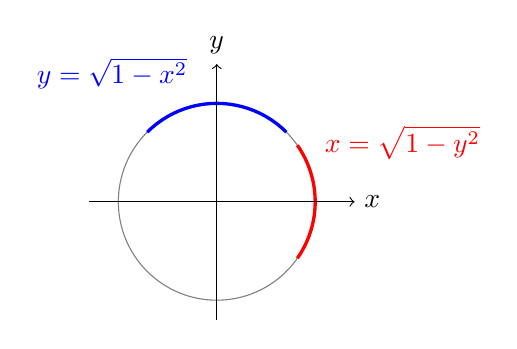
\begin{tikzpicture}[scale=1.25]
\draw[gray] (0,0) circle(1);
\draw[blue,very thick] plot[domain=45:135,samples=25] ({cos(\x)},{sin(\x)});
\draw[red,very thick] plot[domain=-35:35,samples=25] ({cos(\x)},{sin(\x)});
\draw[->] (-1.3,0)--(1.4,0) node[right] {$x$};
\draw[->] (0,-1.2)--(0,1.4) node[above] {$y$};
\node[blue,above left] at (-.2,1.05) {$y=\sqrt{1-x^2}$};
\node[red,right] at (1,.6) {$x=\sqrt{1-y^2}$};
\end{tikzpicture}
\end{minipage}\hfill
\begin{minipage}{0.45\linewidth}
Near the north pole the circle is a graph over $x$; near the rightmost
point it is a graph over $y$. Neither graph covers the whole circle.
The same choice of a nonzero partial derivative gives local graph
descriptions of the regular conics above.
\end{minipage}
\end{center}

\end{example}

\begin{example}[Two dependent variables in an implicit system]
Consider
\[
f(x,y,z)=(y+z-x,\ y-z+x^2).
\]
At $(0,0,0)$ the matrix of derivatives in $(y,z)$ is
$\left(\begin{matrix}1&1\\1&-1\end{matrix}\right)$,
of determinant $-2$. Thus both $y$ and $z$ can be solved as smooth
functions of the one independent variable $x$. Directly adding and
subtracting the equations gives
$y(x)=(x-x^2)/2$, $z(x)=(x+x^2)/2$.
At zero the implicit derivative formula yields
$ (y'(0),z'(0))^{\mathsf T}=(1/2,1/2)^{\mathsf T}$,
which agrees with the explicit solution. The invertible object is the
entire dependent-variable block, not one selected partial derivative.
\end{example}
\begin{center}
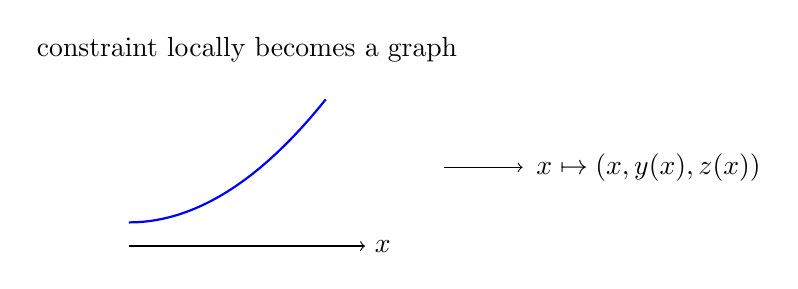
\begin{tikzpicture}
\draw[->] (0,0)--(3,0) node[right] {$x$};
\draw[blue,thick,domain=0:2.5] plot(\x,{.25*\x*\x+.3});
\node at (1.5,2.5) {constraint locally becomes a graph};
\draw[->] (4,1)--(5,1); \node at (6.6,1) {$x\mapsto(x,y(x),z(x))$};
\end{tikzpicture}
\end{center}
\subsection{Analytic refinement: Lagrange inversion (optional)}
The implicit theorem gives a local solution. When the data are analytic,
Lagrange inversion gives its Taylor coefficients explicitly. Analyticity
is essential here: the Implicit Function Theorem alone does not assert it.

\begin{theorem}[Analytic Lagrange inversion; stated result]\label{thm:lagrange-inversion}
Let $\phi$ be real analytic near $0$, with $\phi(0)\ne0$. There is a
unique real analytic solution $w(z)$ near $0$, with $w(0)=0$, of
$w=z\phi(w)$. If $h$ is analytic near $0$, then
\[
[z^n]h(w(z))=\frac1n[t^{n-1}]h'(t)\phi(t)^n\qquad(n\geq1).
\]
Here $[t^j]$ denotes the coefficient of $t^j$ in a power series. In particular,
\[
w(z)=\sum_{n\geq1}\frac{z^n}{n!}
 \left[\frac{d^{n-1}}{dt^{n-1}}\phi(t)^n\right]_{t=0}.
\]
\end{theorem}
This optional analytic result, including convergence, is used without proof;
it is not needed below. See \cite[\S2.1 and \S2.6]{gessel-lagrange}
for the coefficient formulations and \cite{sokal-implicit} for analytic
implicit solutions. No complex integration is needed for its use here.
The smooth implicit theorem applied to $f(z,w)=w-z\phi(w)$, whose
$w$ derivative at $(0,0)$ is $1$, already supplies the unique smooth local
solution. The additional analytic theorem identifies that solution with
a convergent series; it is this extra conclusion that licenses Taylor
reconstruction.

\begin{example}[A computable implicit series]
Take $\phi(t)=1+t^2$ and $h(t)=t$. The coefficient rule gives zero in
even degrees, and in degree $2j+1$ gives
$\binom{2j+1}{j}/(2j+1)$. Hence
\[
w=z+z^3+2z^5+5z^7+\cdots.
\]
The first coefficients can also be derived directly: substituting
$w=a_1z+a_2z^2+\cdots$ into $w=z+zw^2$ gives
$a_1=1$, $a_2=0$, $a_3=1$, $a_4=0$, and $a_5=2$.
Convergence also follows from an elementary coefficient bound. Write
\[
c_j=\frac{1}{2j+1}\binom{2j+1}{j}
=\frac{1}{j+1}\binom{2j}{j}.
\]
The finite binomial theorem gives
$0\leq c_j\leq\binom{2j}{j}\leq 2^{2j}=4^j$. Thus, for $|z|<1/2$,
\[
\sum_{j=0}^{\infty}c_j|z|^{2j+1}
\leq |z|\sum_{j=0}^{\infty}(4|z|^2)^j
=\frac{|z|}{1-4|z|^2}.
\]
The algebraic solution $w=(1-\sqrt{1-4z^2})/(2z)$, with its removable
value $0$ at zero, provides an independent consistency check.
\end{example}

\section{Rank and Local Normal Forms}
\label{sec:rank-normal-forms}
An invertible derivative preserves all directions. More generally its
rank counts how many independent first-order output directions remain.
Constant rank lets us turn this linear information into local coordinates.

\begin{definition}[Rank of a map]\label{def:map-rank}
For a $C^1$ map $f:U\subseteq\R^n\to\R^m$ on an open set, define
\[
\operatorname{rank}_a f=\operatorname{rank}Df(a)
=\dim\operatorname{im}Df(a)=\operatorname{rank}J_f(a).
\]
The map has \textbf{constant rank $r$} on a set if this number equals $r$
at every point of that set.
\end{definition}
\begin{lemma}[Persistence of a nonzero minor]\label{lem:rank-persistence}
If $\operatorname{rank}Df(a)=r$, then $\operatorname{rank}Df(x)\geq r$
on a neighborhood of $a$.
\end{lemma}
\begin{proof}
For $r=0$ the claim is automatic. Otherwise \cref{prop:rank-minors}
supplies an $r\times r$ minor with determinant $d\ne0$. Its determinant is continuous in $x$, since the
entries of $Df$ are continuous and a determinant is a polynomial in them.
On a neighborhood where its difference from $d$ is less than $|d|/2$,
that minor is nonzero, so the rank is at least $r$.
\end{proof}

\begin{theorem}[Constant Rank Theorem]\label{thm:constant-rank}
Let $f:U\subseteq\R^n\to\R^m$ be $C^k$, $1\leq k\leq\infty$,
and suppose its rank is constantly $r$ near $a$. There are local
$C^k$ diffeomorphisms $\phi$ near $a$ and $\psi$ near $f(a)$, taking
these points to zero, for which
\[
(\psi\circ f\circ\phi^{-1})(u_1,\ldots,u_n)
=(u_1,\ldots,u_r,0,\ldots,0)
\]
on a neighborhood of zero.
\end{theorem}
\begin{proof}
We first use $r$ outputs as source coordinates, then remove the dependence
of the remaining outputs on those coordinates. If $r=0$, the derivative
vanishes on a ball about $a$; the mean-value estimate makes $f$ constant
there. Translations in source and target give the assertion. Assume $r>0$.
Translate $a$ and $f(a)$ to zero and permute coordinates so that the
first $r$ rows and columns form an invertible submatrix. Write $x=(s,t)$,
$s\in\R^r$, $t\in\R^{n-r}$, and set
\[
A(s,t)=(f_1(s,t),\ldots,f_r(s,t),t).
\]
Its derivative at zero is block triangular with the chosen submatrix and
$I_{n-r}$ on its diagonal. The inverse function theorem gives a local
$C^k$ diffeomorphism $A$. Restrict its image to a product of open boxes
$B\times D$ centered at zero, and its source to the inverse image of that
product. Then
\[
f\circ A^{-1}(u,v)=(u,g(u,v)),\qquad
D(f\circ A^{-1})=
\begin{pmatrix}I_r&0\\D_ug&D_vg\end{pmatrix}.
\]
Right multiplication by the invertible $DA^{-1}$ preserves rank, so this
matrix has rank $r$. Its first $r$ columns are independent. Every other
column has zero first block and must be their linear combination; the top
block of that combination is exactly its coefficient vector. That vector
must therefore be zero. The entire column vanishes, proving $D_vg=0$.
For fixed $u$, the segment between any two points of $D$ stays in $D$;
the mean-value estimate gives $g(u,v)=g(u,0)=h(u)$.
If there are no $v$ coordinates this assertion simply defines $h=g$.

On the open target set $B\times\R^{m-r}$ the map
\[
\psi_0(y,z)=(y,z-h(y))
\]
is a $C^k$ diffeomorphism, with inverse $(y,z)\mapsto(y,z+h(y))$.
It sends $(u,h(u))$ to $(u,0)$. Taking $\phi=A$ and $\psi=\psi_0$
in these translated and permuted coordinates gives the desired formula.
Composing with the original translations and permutations gives actual
coordinate diffeomorphisms for the original map and base points.
Empty blocks when $r=m$ are omitted.
\end{proof}
The principal special cases are
\[
\begin{array}{ccl}
r=n=m&\Rightarrow&\text{inverse-function normal form},\\
r=m\leq n&\Rightarrow&\text{projection normal form},\\
r=n\leq m&\Rightarrow&\text{inclusion normal form}.
\end{array}
\]
\begin{definition}[Immersion and submersion]\label{def:immersion-submersion}
A $C^1$ map $f:U\subseteq\R^n\to\R^m$ is an \textbf{immersion at $a$}
if $Df(a)$ is injective, equivalently $\operatorname{rank}_a f=n$.
It is a \textbf{submersion at $a$} if $Df(a)$ is surjective,
equivalently $\operatorname{rank}_a f=m$. These require $n\leq m$ and
$m\leq n$, respectively. It is an immersion or submersion on $U$ if the
corresponding condition holds at every point.
\end{definition}
The persistence lemma makes either full-rank condition hold on a
neighborhood, so the Constant Rank Theorem applies. Projection
$(x,y)\mapsto x$ is a submersion, and inclusion $x\mapsto(x,0)$ is an
immersion. The terminology is Euclidean here. Chapter~13 constructs the intrinsic
differential needed to formulate the manifold notions, developed in
Appendix~\ref{app:submanifolds}.
\begin{example}[A normal form and a rank drop]
The map $f(x,y)=(x+y,(x+y)^2)$ has rank one everywhere.
The coordinate changes $\phi(x,y)=(x+y,y)$ and
$\psi(u,v)=(u,v-u^2)$ give $\psi f\phi^{-1}(u,v)=(u,0)$.
In contrast, $(x,y)\mapsto(x,xy)$ has determinant $x$ and rank drops
from two to one on $x=0$; there is no constant-rank neighborhood there.
\end{example}

\subsection{Submersions, Regular Level Sets, and Multipliers}
\label{sec:ift-consequences}
The submersion normal form describes level sets as coordinate planes.
The implicit graph description also identifies their tangent directions directly.
\begin{corollary}[Regular level sets and tangent directions]\label{cor:regular-level-set}
Let $f:U\subseteq\R^n\to\R^m$ be $C^1$ on open $U$, $m\leq n$, and suppose
$f(a)=c$, $\operatorname{rank}Df(a)=m$. Near $a$, the level set
$f^{-1}(c)$ is a $C^1$ graph of $n-m$ variables. Its tangent directions,
defined as velocities at $a$ of $C^1$ curves in the level set, are exactly
$\ker Df(a)$.
\end{corollary}
\begin{proof}
The images of the coordinate basis vectors span $\R^m$; select $m$ of
them forming a basis and reorder these as dependent coordinates $y$.
The remaining coordinates are $x\in\R^{n-m}$, and $D_yf(a)$ is invertible.
Apply the implicit theorem to $f(x,y)-c$ to obtain $y=\phi(x)$ locally.
A curve $\gamma$ in the level set satisfies $Df(a)\gamma'(0)=0$ by
the chain rule. Conversely write a kernel vector as $(u,v)$. The equation
$D_xf(a)u+D_yf(a)v=0$ gives $v=D\phi(a_x)u$.
The curve $(a_x+tu,\phi(a_x+tu))$ has exactly this velocity and stays
in the level set for small $t$. If $m=n$, the graph has zero free
variables and the local level set is a single point; its only velocity is zero.
\end{proof}
Writing $T_af^{-1}(c)$ for these curve velocities, the conclusion is
\[
T_af^{-1}(c)=\ker Df(a).
\]
Thus $m$ independent equations leave local dimension $n-m$.
For scalar $f$, $\nabla f(a)\ne0$ gives an $(n-1)$-dimensional graph and
$\ker Df(a)=\{v:\nabla f(a)\cdot v=0\}$. This makes the gradient normal
to the constraint and prepares the multiplier condition below.

\begin{remark}[Equations, graphs, and parametrizations]
The classical descriptions $y=f(x)$, $f(x,y)=0$, and
$(x,y)=\gamma(t)$ become, in higher dimensions, a graph $y=\varphi(x)$,
a level set $f(x)=c$, and a parametrization $x=\sigma(u)$.
The implicit theorem turns a regular equation locally into a graph;
the constant-rank theorem gives its coordinate normal form. In Chapter~13,
the inverse of a chart will provide the corresponding local parametrization.
For a regular scalar level surface in $\R^3$, the affine tangent plane is
\[
\nabla f(a)\cdot(x-a)=0,
\qquad T_a(f^{-1}(c))=\ker Df(a).
\]
The gradient is the Euclidean representative of the derivative covector.
For $a,b,c,R,p>0$, useful familiar models are
\[
\begin{array}{ll}
x^2/a^2+y^2/b^2=1&\text{ellipse},\\
x^2/a^2-y^2/b^2=1&\text{hyperbola},\\
y=x^2/(4p)&\text{parabola},\\
x^2/a^2+y^2/b^2+z^2/c^2=1&\text{ellipsoid},\\
x^2+y^2=R^2&\text{cylinder},\\
x^2+y^2=z^2&\text{cone},\\
z=x^2+y^2&\text{elliptic paraboloid}.
\end{array}
\]
Their defining gradients are nonzero on these sets, except at the cone's
vertex. Thus the regular-level argument applies away from that vertex.
Scaling turns the ellipsoid into a sphere; cylindrical coordinates simplify
the cylinder and cone. These coordinate choices will also simplify integrals.
\end{remark}
% Original vector figure for Version 3.9.0.
\begin{figure}[htbp]
\centering
\begin{tikzpicture}[font=\small,>=Stealth,line width=.65pt]
\begin{scope}[x={(1cm,-.28cm)},y={(-.65cm,-.38cm)},z={(0cm,.8cm)}]
\filldraw[fill=orange!15,draw=orange!70!black] (-1.2,-1.2,1)--(1.2,-1.2,1)--(1.2,1.2,1)--(-1.2,1.2,1)--cycle;
\foreach \v in {-.9,-.45,0,.45,.9}{\draw[blue!70] plot[domain=-.9:.9,samples=30] (\x,\v,{1-.35*(\x*\x+\v*\v)});}
\foreach \u in {-.9,-.45,0,.45,.9}{\draw[blue!70] plot[domain=-.9:.9,samples=30] (\u,\x,{1-.35*(\x*\x+\u*\u)});}
\fill (0,0,1) circle(2pt) node[left] {$a$};
\draw[->,red!80!black,thick] (0,0,1)--(0,0,2.6) node[above] {$\nabla f(a)$};
\end{scope}
\node[right,align=left] at (2.4,.2) {$f(x,y,z)=c$\\$T_a(f^{-1}(c))=\ker Df(a)$};
\end{tikzpicture}
\caption{The regular level surface has tangent direction space $\ker Df(a)$. Its affine tangent plane passes through $a$; the gradient is normal to it.}\label{fig:implicit-surface}
\end{figure}

% Original vector figure for Version 3.9.0.
\begin{figure}[htbp]
\centering
\begin{tikzpicture}[font=\small,>=Stealth,line width=.65pt]
\begin{scope}[xshift=-3cm]
\draw[->,gray] (-1.3,0)--(1.3,0);\draw[->,gray] (0,-1)--(0,1);
\draw[blue,thick] (0,0) ellipse(1 and .65);
\node[below] at (0,-1) {ellipse};
\end{scope}
\begin{scope}[xshift=.1cm]
\draw[->,gray] (-1.3,0)--(1.3,0);\draw[->,gray] (0,-1)--(0,1);
\draw[blue,thick] plot[domain=-.8:.8,samples=35] ({sqrt(.35+\x*\x)},\x);
\draw[blue,thick] plot[domain=-.8:.8,samples=35] ({-sqrt(.35+\x*\x)},\x);
\node[below] at (0,-1) {hyperbola};
\end{scope}
\begin{scope}[xshift=3.2cm]
\draw[->,gray] (-1.2,0)--(1.2,0);\draw[->,gray] (0,-.2)--(0,1.1);
\draw[blue,thick] plot[domain=-1:1,samples=35] (\x,{\x*\x});
\node[below] at (0,-1) {parabola};
\end{scope}
\end{tikzpicture}
\caption{Three regular conics. Their equations become local graphs wherever the corresponding partial derivative is nonzero; a vertical tangent requires solving for the other variable.}\label{fig:conics-quadrics}
\end{figure}

The auxiliary map already used in the proof,
$h(x,y)=(x,f(x,y))$, is a local diffeomorphism when $D_yf(a)$ is invertible.
In coordinates $(x,z)=h(x,y)$, the equation
$f(h^{-1}(x,z))=z$ says that $f$ becomes projection onto the second block.
This is the local submersion form supplied by the same proof.

If $f:U\to\R^n$ is $C^1$ with invertible derivative everywhere, the inverse
theorem makes it a local diffeomorphism at every point. It is an open map:
for any open $V\subseteq U$, restrict a local inverse neighborhood at each
$x\in V$; its intersection with $V$ has open image under that local
homeomorphism, and these images cover $f(V)$. This does not give global
injectivity, as the earlier periodic map $(x,y)\mapsto(e^x\cos y,e^x\sin y)$
demonstrates: $y$ and $y+2\pi$ have the same image.

Continuity of the determinant also shows that $\det Df(a)\ne0$ has
constant nonzero sign on a sufficiently small neighborhood of $a$.
Positive sign means locally orientation preserving; negative sign means
locally orientation reversing. Chapters~12--13 use its magnitude and sign
for their different integration purposes.

Finally the implicit formula is a statement of smooth dependence on
parameters: if $f(t,y)=0$ and $D_yf(t_0,y_0)$ is invertible, the nearby
solution $y=\phi(t)$ has the regularity of $f$ and
$D\phi(t)=-(D_yf(t,\phi(t)))^{-1}D_tf(t,\phi(t))$.
For $f(t,y)=y^2-t$ at $(1,1)$ this selects the positive branch
$\phi(t)=\sqrt t$ near $1$, and $\phi'(t)=1/(2\phi(t))$.
The negative branch illustrates why the conclusion is local to the chosen solution.


\begin{theorem}[Lagrange multipliers for one constraint]
\label{thm:lagrange-multipliers}
Let $f,g:U\subseteq\R^n\to\R$ be of class $C^1$.  Suppose that $a$ is a
local extremum of $f$ subject to
\[
g(x)=c,
\]
with $g(a)=c$, and that $\nabla g(a)\ne0$.  Then there is $\lambda\in\R$ such that
\[
\nabla f(a)=\lambda\nabla g(a).
\]
\end{theorem}
\begin{proof}
By \cref{cor:regular-level-set}, the level set $g=c$ is locally a
$C^1$ graph with tangent space $T=\ker Dg(a)$. Every tangent vector
is the velocity of a curve in that graph. The restriction of $f$ has
a local extremum, so the one-variable derivative along each such curve
is zero. The chain rule gives $Df(a)v=0$ for every $v\in T$.
Thus $Df(a)$ vanishes on $\ker Dg(a)$. Write $\ell=Dg(a)$ and $m=Df(a)$.
Choose $w$ with $\ell(w)=1$; this is possible by rescaling a vector
where the nonzero functional $\ell$ does not vanish. Every vector splits as
\[
v=\bigl(v-\ell(v)w\bigr)+\ell(v)w,
\quad v-\ell(v)w\in\ker\ell.
\]
Applying $m$ kills the first summand, giving $m(v)=m(w)\ell(v)$.
Thus $m=m(w)\ell$ as functionals. Geometrically the allowed tangent
directions lie in the constraint kernel; a constrained extremum has no
first-order change in any such direction. With the Euclidean inner
product the two representing gradients are parallel.
Thus $\lambda=m(w)$ gives the stated gradient equation.
\end{proof}

\begin{example}[Why the defining equation must be regular]
Let $g(x,y)=y^2$ and $f(x,y)=x^2+y$. On $g=0$ we have $y=0$ and
$f(x,0)=x^2$, so zero is a strict constrained minimum. But
$\nabla g(0)=0$ while $\nabla f(0)=(0,1)$; no multiplier equation is
possible. The equivalent defining equation $y=0$ has nonzero gradient
and gives multiplier $1$. Regularity concerns the chosen equation,
not merely its geometric zero set.
\end{example}

\begin{example}[Extrema of $xy$ on the unit circle]
To maximize or minimize
\[
f(x,y)=xy
\]
subject to $g(x,y)=x^2+y^2=1$, observe that
\[
\nabla f=(y,x),
\qquad
\nabla g=(2x,2y).
\]
The Lagrange equations are
\[
(y,x)=\lambda(2x,2y),
\qquad x^2+y^2=1.
\]
They give $\lambda=1/2$ and $y=x$, or $\lambda=-1/2$ and $y=-x$.
Thus $f=1/2$ at
\[
\left(\frac1{\sqrt2},\frac1{\sqrt2}\right),
\qquad
\left(-\frac1{\sqrt2},-\frac1{\sqrt2}\right),
\]
and $f=-1/2$ at the two points with $y=-x$.  These are respectively the
maximum and minimum, as also follows from $2\abs{xy}\leq x^2+y^2=1$.
\end{example}

\begin{remark}[How to recognize which theorem to use]
For a map $f:\R^n\to\R^n$, a question about a local inverse calls for
computing $Df(a)$ and checking that it is invertible (equivalently, that its
determinant is nonzero).  For equations $f(x,y)=0$ and a request to solve for
the $y$ variables, compute the block $D_yf(a,b)$ instead.  In either case,
the result concerns neighborhoods of the specified point, not a global
inverse or a global parametrization.
\end{remark}


\subsection{Dimension consequences}
The normal form detects lost source directions. A different covering
argument will detect when a source has too few dimensions to fill an open
target.
\begin{theorem}[More source dimensions prevent injectivity]\label{thm:dimension-noninjective}
If $U\subseteq\R^n$ and $V\subseteq\R^m$ are nonempty open sets,
$n>m$, and $f:U\to V$ is $C^1$, then $f$ is not injective.
\end{theorem}
\begin{proof}
The set of attained ranks is a nonempty subset of the finite set
$\{0,\ldots,m\}$. It therefore has a largest member $r$, attained at
some $a\in U$. By \cref{lem:rank-persistence} the rank is at least $r$
near $a$; maximality makes it equal to $r$ there.
The Constant Rank Theorem supplies coordinates in which $f$ is
$(u_1,\ldots,u_n)\mapsto(u_1,\ldots,u_r,0,\ldots,0)$.
Since $r\leq m<n$, a small change in coordinate $u_{r+1}$ stays in
the open coordinate neighborhood and leaves the image unchanged. The
inverse source coordinate map gives two distinct points with the same
$f$ value, because the target coordinate map is injective.
\end{proof}
\begin{theorem}[Fewer source dimensions prevent surjectivity]\label{thm:dimension-nonsurjective}
Under the same open-set and $C^1$ hypotheses, if $n<m$, then $f$ is
not surjective.
\end{theorem}
The proof is deferred to \cref{thm:lower-dimensional-image} in Chapter~12.
It uses small-box volume bounds and compactness, not the Constant Rank
Theorem. In particular, a countable union of Jordan-null sets need not
be Jordan-null; that inference will not be used.
\begin{proposition}[Diffeomorphisms preserve dimension]\label{prop:diffeomorphism-dimension}
A $C^1$ diffeomorphism between nonempty open subsets of $\R^n$ and
$\R^m$ requires $n=m$.
\end{proposition}
\begin{proof}
Writing $g=f^{-1}$, the chain rule at $a$ and $f(a)$ gives
\[
Dg(f(a))Df(a)=I_{\R^n},\qquad Df(a)Dg(f(a))=I_{\R^m}.
\]
Thus $Df(a):\R^n\to\R^m$ is a linear isomorphism, so $n=m$.
\end{proof}

\subsection{Primitive diffeomorphisms and local factorization}
Elementary coordinate operations have nonlinear counterparts: one output
coordinate changes while the others remain available as parameters.
\begin{definition}[Primitive map]\label{def:primitive-map}
A $C^k$ map on an open subset of $\R^n$ is \textbf{primitive} if for
some $i$ it has the form
\[
q(x)=(x_1,\ldots,x_{i-1},p(x),x_{i+1},\ldots,x_n).
\]
A primitive diffeomorphism is such a map that is a diffeomorphism onto
an open image. Coordinate permutations are treated separately.
\end{definition}
Expanding its determinant along the unchanged rows gives
$\det Dq=\partial_i p$. Thus $\partial_i p(a)\ne0$ makes $q$ a local
$C^k$ diffeomorphism at $a$ by the inverse theorem. To see why one
product box suffices, write the changed coordinate last:
$q(x',t)=(x',p(x',t))$. Continuity keeps $\partial_t p$ of one sign
on a sufficiently small open product box $B$ around $a$. For fixed $x'$,
the mean value theorem makes $t\mapsto p(x',t)$ strictly monotone.
If $q(x',t)=q(y',s)$, the unchanged coordinates give $x'=y'$, and
strict monotonicity then gives $t=s$. Thus $q$ is injective on all of $B$.
At every point of $B$ its derivative is invertible, so the inverse
function theorem gives an open image neighborhood and a $C^k$ local
inverse. These image neighborhoods cover $q(B)$, making it open.
On overlaps the local inverses agree because injectivity permits only
one preimage in $B$. They therefore define a $C^k$ inverse
$q^{-1}:q(B)\to B$. Solving a primitive map requires solving only one
scalar equation.

\begin{theorem}[Local primitive factorization]\label{thm:primitive-factorization}
Let $f:U\subseteq\R^n\to\R^n$ be $C^k$, $k\geq1$, with $Df(a)$
invertible. There is a source neighborhood $N$ on which, after a
permutation of output coordinates, $f$ is a composition of $n$ primitive
$C^k$ diffeomorphisms between open sets. This is a local assertion.
\end{theorem}
The coordinate replacements can be chosen successively. Once the first
$j-1$ outputs equal their input coordinates, invertibility forces some
remaining output to detect the $j$th source direction. Using that output
as a new coordinate makes one more coordinate exact.
\begin{proof}
By the inverse function theorem, restrict $f_0=f$ to a local $C^k$
diffeomorphism near $a_0=a$. Suppose $f_{j-1}$ is a local diffeomorphism
near $a_{j-1}$ whose first $j-1$ components are $x_1,\ldots,x_{j-1}$.
Invertibility gives
\[
Df_{j-1}(a_{j-1})e_j\ne0.
\]
Its first $j-1$ components are zero, since $\partial_j x_l=0$ for
$l<j$. Thus some $i\geq j$ satisfies
$\partial_jf_{j-1,i}(a_{j-1})\ne0$. Choose an output permutation
$\tau_j$ fixing coordinates $1,\ldots,j-1$ and bringing this component
to position $j$. Put $g_j=\tau_j\circ f_{j-1}$ and define
\[
q_j(x)=(x_1,\ldots,x_{j-1},g_{j,j}(x),x_{j+1},\ldots,x_n).
\]
The scalar function $g_{j,j}$ is component $j$ of the permuted residual map.
Since $\det Dq_j(a_{j-1})=\partial_jg_{j,j}(a_{j-1})\ne0$, the
inverse function theorem makes $q_j$ a primitive $C^k$ diffeomorphism
on a smaller neighborhood. Set
\[
a_j=q_j(a_{j-1}),\qquad
f_j=g_j\circ q_j^{-1}=\tau_j\circ f_{j-1}\circ q_j^{-1}.
\]
For $y=q_j(x)$, the first $j-1$ components of $g_j(x)$ are
$x_l=y_l$, and its $j$th component is $g_{j,j}(x)=y_j$. Consequently
\[
f_j(y)=(y_1,\ldots,y_j,f_{j,j+1}(y),\ldots,f_{j,n}(y)).
\]
It is again a local diffeomorphism, now near $a_j$, so induction continues.

All these constructions take place on open neighborhoods. At each stage
restrict the current neighborhood so that the next $q_j$ and its inverse
are defined, and pull that restriction back through the preceding
primitive factors to a neighborhood of $a$. Previously constructed maps
remain diffeomorphisms when restricted to these open subsets. There are
only finitely many stages, so this gives one final source neighborhood
$N$ on which every factor and inverse in the composite is defined.

At the last stage $f_n=\mathrm{id}$. Each $\tau_j$ fixes the coordinates
already made exact, and their composite is the single permutation
$\sigma=\tau_n\circ\cdots\circ\tau_1$. Iterating the defining identities
on the final neighborhoods gives
\[
\mathrm{id}=f_n
=\sigma\circ f\circ q_1^{-1}\circ\cdots\circ q_n^{-1}.
\]
Composing on the right with the primitive factors in reverse order yields
\[
\sigma\circ f|_N=q_n\circ\cdots\circ q_1.
\]
\end{proof}
\begin{example}[Two successive coordinate replacements]
For $f(x,y)=(x+y,y+(x+y)^2)$, take
$q_1(x,y)=(x+y,y)$ and $q_2(u,v)=(u,v+u^2)$.
Then $f=q_2\circ q_1$ and both primitive determinants equal one.
\end{example}
Chapter~12 will reduce a local change of variables to repeated
one-coordinate substitutions through \cref{thm:primitive-factorization};
compare the structural treatments in
\cite{knapp-basic-real,munkres-analysis,rudin-pma}.

\subsection{Finite Euclidean localization}
Compact support makes finitely many local formulas enough. We now build
smooth weights that assemble them without counting overlaps twice.
\phantomsection\label{def:euclidean-function-support}
For a function on an open set $G$, its support is the closure in $G$ of
its nonzero set; $C_c^\infty(G)$ denotes smooth functions whose support
is compact in $G$. Such functions extend smoothly by zero to $\R^n$.

\begin{lemma}[Euclidean cutoff]\label{lem:euclidean-cutoff}\label{cor:compact-cutoff}
If $K\subset G\subseteq\R^n$, $K$ is compact, and $G$ is open, there
is $\chi\in C_c^\infty(G)$ with $0\leq\chi\leq1$ and $\chi=1$
on a neighborhood of $K$.
\end{lemma}
\begin{proof}
For empty $K$ use zero. From \cref{thm:smooth-cutoff} form
\[
s(t)=\frac{\theta(t)}{\theta(t)+\theta(1-t)}.
\]
The denominator is positive everywhere. Thus $s$ is smooth, lies in
$[0,1]$, equals zero for $t\leq0$, and equals one for $t\geq1$.
For each $a\in K$ choose $r_a>0$ with $\overline B(a,2r_a)\subset G$.
Finitely many $B(a_j,r_j)$ cover $K$. Define
\[
b_j(x)=s\left(\frac{4r_j^2-\|x-a_j\|^2}{3r_j^2}\right),
\qquad \chi(x)=1-\prod_j(1-b_j(x)).
\]
The function $b_j$ is one on $\overline B(a_j,r_j)$ and supported in
$\overline B(a_j,2r_j)$. Hence $\chi$ has the required range, equals
one on the union of the smaller open balls, and has compact support in
the finite union of the larger closed balls inside $G$.
\end{proof}

\begin{theorem}[Finite Euclidean partition of unity]\label{thm:finite-euclidean-pou}
If a compact $K\subseteq\R^n$ is covered by open sets $U_1,\ldots,U_N$,
there are smooth $\rho_i:\R^n\to[0,1]$ with compact support in $U_i$
and $\sum_i\rho_i=1$ on a neighborhood of $K$.
\end{theorem}
\begin{proof}
\textbf{Strategy.} Assign each cutoff the portion not already assigned;
the finite product identity telescopes.

For each point of $K$ choose a ball about it whose doubled closed ball
lies in one of the $U_i$, and choose a finite subcover by the smaller
balls. Let $K_i$ be the union of the smaller closed balls assigned to
$U_i$ (possibly empty). Then $K_i$ is compact in $U_i$, and their
interiors cover $K$. Choose $\chi_i$ by \cref{lem:euclidean-cutoff}, equal
to one near $K_i$ and compactly supported in $U_i$.
Define globally
\[
\rho_i=\chi_i\prod_{j<i}(1-\chi_j),\qquad
p_0=1,\qquad p_i=\prod_{j=1}^i(1-\chi_j).
\]
Then $\rho_i=p_{i-1}-p_i$, so
\[
\sum_{i=1}^N\rho_i=1-\prod_{i=1}^N(1-\chi_i).
\]
Near every point of $K$, at least one $\chi_i$ equals one. The sum is
therefore one on an open neighborhood of $K$. Each $\rho_i$ is globally
smooth, $0\leq\rho_i\leq1$, and
$\operatorname{supp}\rho_i\subseteq\operatorname{supp}\chi_i\subset U_i$
is compact. Each successive cutoff receives the portion not already
assigned by earlier cutoffs. The order dependence is harmless for existence.
\end{proof}
The finite Euclidean construction is all that Chapter~12 needs. Chapter~13
replaces the finite compact situation by locally finite covers of manifolds.

\section*{Exercises}
\addcontentsline{toc}{section}{Exercises}
The first exercises practice the computational tests and conic geometry;
the remaining problems range across the chapter.
\begin{exercise}
For $f(x,y)=xy+y^2$, $a=(1,2)$, and $v=(2,-1)$, compute $(df)_a$,
express it in $\dd x,\dd y$, and evaluate $(df)_a(v)$. For
$\gamma(t)=(1+2t,2-t)$, compare this value with $(f\circ\gamma)'(0)$
computed directly and by the chain rule.
\end{exercise}
\begin{exercise}
Find polar coordinates for $(-\sqrt3,-1)$ with $0\leq\theta<2\pi$.
Explain why $\arctan(y/x)$ alone selects the wrong quadrant.
\end{exercise}
\begin{exercise}
For $f(x,y)=xy/\sqrt{x^2+y^2}$, extended by zero, decide which of continuity,
coordinate partials, all two-sided directional derivatives, and differentiability
hold at zero. Explain why the direction $(1,1)$ is decisive.
\end{exercise}
\begin{exercise}
Estimate directly the normalized remainder of $x^2+xy+2y^2$ at an arbitrary
point. Find the tangent line and a unit normal to $x^2/4+y^2=1$ at
$(\sqrt2,1/\sqrt2)$.
\end{exercise}



\begin{exercise}
For
\[
f(x,y)=(x^2y,\sin(x+y)),
\]
compute $Df(x,y)$ and $Df(x,y)(u,v)$.
\end{exercise}

\begin{exercise}
Give a function from $\R^2$ to $\R$ with both partial derivatives at the
origin but which is not differentiable there.
\end{exercise}

\begin{exercise}
Prove that a linear map between finite-dimensional normed spaces is
differentiable everywhere and is its own derivative.
\end{exercise}

\begin{exercise}
Prove directly from the definition that differentiability at $a$ implies
continuity at $a$.
\end{exercise}

\begin{exercise}
Use \cref{thm:multivariable-mvt} to prove that a $C^1$ map with zero
derivative on a convex open set is constant.
\end{exercise}

\begin{exercise}
Compute the Hessian of
\[
x^3+xy^2-3x
\]
and classify its critical points.
\end{exercise}

\begin{exercise}
Apply Taylor's theorem to find the quadratic approximation of
\[
e^x\sin y
\]
at the origin.
\end{exercise}

\begin{exercise}
Give a function with unequal mixed partial derivatives at the origin and
explain why \cref{thm:schwarz} does not apply.
\end{exercise}

\begin{exercise}
Use the contraction mapping theorem to prove that
\[
x=\cos x
\]
has a unique solution in
\[
[0,1].
\]
\end{exercise}

\begin{exercise}
Let $A$ be a matrix with
\[
\norm{I-A}_{\mathrm{op}}<1.
\]
Show that
\[
x_{k+1}=(I-A)x_k+b
\]
converges to the unique solution of
\[
Ax=b.
\]
\end{exercise}

\begin{exercise}
Apply the inverse function theorem to
\[
f(x,y)=(e^x\cos y,e^x\sin y)
\]
at $(0,0)$ and compute the derivative of its local inverse at $(1,0)$.
\end{exercise}

\begin{exercise}
Near $(0,1)$, use the implicit function theorem on
\[
x^2+y^2+xy=1
\]
to solve for $y$ as a $C^1$ function of $x$ and find its derivative at zero.
\end{exercise}

\begin{exercise}
Explain why
\[
y^2=x^3
\]
has a full local zero set that is not the graph of one function on an
open interval containing zero. Separately show that its one-sided branches
$y=\pm x^{3/2}$, $x\geq0$, are $C^1$ up to the origin.
\end{exercise}

\begin{exercise}
For $f(x,y)=\log(1+x)+y^2$ near zero, compute $Df(0)$ and $D^2f(0)$ and write
the second-order Peano formula. Distinguish its quadratic term from the
bilinear second derivative evaluated on two different vectors.
\end{exercise}
\begin{exercise}
Iterate $T(x)=\cos x/2$ on $[0,1]$. Check self-map, contraction,
and completeness, then give an a priori error bound after ten steps
starting at zero. Which bound uses the last observed step?
\end{exercise}
\begin{exercise}
For $f(x,y,z)=(y+z-x,y-z+x^2)$ calculate the implicit derivative at
$x=1$ from the block formula and the explicit solution. Identify its
source dimension and target dimension.
\end{exercise}
\begin{exercise}
At the origin compare the second-order tests for $x^2+2y^2$,
$x^2-y^2$, and $x^2+y^4$. In the last case, explain why the theorem
is inconclusive even though the definition decides the minimum.
\end{exercise}

\begin{exercise}
For $T(x,y,z)=(x+2y+z,y-z)$ choose $x$ independent and $(y,z)$ dependent.
Compute $-T_y^{-1}T_x$ and parametrize the kernel by its graph map.
\end{exercise}
\begin{exercise}
Find the ranks and rank-drop sets of $(x,y)\mapsto(x,xy)$ and
$(x,y,z)\mapsto(x+y,z)$. Identify the submersions and immersions.
\end{exercise}
\begin{exercise}
For $f(x,y)=(x+y,y+(x+y)^2)$ compute the two primitive inverses and
verify the determinant product. Put $(x+y,(x+y)^2)$ in constant-rank form.
\end{exercise}
\begin{exercise}
Use the transition $s$ from the cutoff proof to construct two smooth
weights subordinate to $(-\infty,2)$ and $(-1,\infty)$ that sum to one.
For $w=z(1+w)^2$, use Lagrange inversion to compute through degree four.
\end{exercise}

\section{Perspective and Transition}

Chapter~12 combines primitive factorization, one-variable substitution,
Fubini, and finite Euclidean localization to transform integrals.
Rank and its normal forms explain the underlying local geometry. In Chapter~13 derivatives transport tangent
directions, while pullbacks transport covectors and forms. Exterior
differentiation and integration then lead to Stokes' theorem.
